\documentclass[a4paper,12pt,headsepline]{scrartcl}

%\part{title}
\usepackage[utf8]{inputenc}
\usepackage{graphicx}
\usepackage{caption,subcaption}
\usepackage[english]{babel}
\usepackage[T1]{fontenc}
\usepackage{geometry}
\usepackage{proof}
\geometry{left=3.5cm, right=2cm, top=2.5cm, bottom=2cm}
\usepackage{hyperref}
%\usepackage[hyphens,obeyspaces,spaces]{url}
\usepackage{fancybox}
\usepackage{amssymb,amsmath,amsthm}
\usepackage{gensymb}
\usepackage[linesnumbered,ruled,vlined,norelsize]{algorithm2e}
%\usepackage[bookmarksnumbered,pdftitle={\titleDocument},hyperfootnotes=false]{hyperref} 
\usepackage{color}
\usepackage{float}

%test
\usepackage[backend=bibtex]{biblatex}
\usepackage{filecontents}

\addbibresource{ref.bib}

\restylefloat{figure}

% Makros
\newenvironment{sketch}{\begin{proof}[Proof (Sketch)]}{\end{proof}}
\newtheorem{theorem}{Theorem}
\newtheorem{assumption}{Assumption}
\newtheorem{lemma}{Lemma}
\newtheorem{remark}{Remark}
\newtheorem{definition}{Definition}
\newtheorem{corollary}{Corollary}
\newcommand{\comment}[1]
{
  \begin{quotation}
    \textcolor{blue}{\underline{Edit:} #1}
  \end{quotation}
}
\newcommand{\TODO}[1]
{
  \begin{quotation}
    \textcolor{red}{\underline{TODO:} #1}
  \end{quotation}
}
\newcommand{\mygraphics}[3][2]{
\begin{figure}[h]
	\centering
	\includegraphics[page=#1]{#2}
	\caption{#3}
\end{figure}
}

% Zeichen 
\newcommand{\Rho}{\ensuremath{\mathcal{O}}}
\newcommand{\ec}{\texttt{ec}}
\newcommand{\NP}{\call{NP}}
\newcommand{\call}[1]{\ensuremath{\mathcal{#1}}}

% neue Kopfzeilen mit fancypaket
\usepackage{fancyhdr} %Paket laden
\pagestyle{fancy} %eigener Seitenstil
\fancyhf{} %alle Kopf- und Fußzeilenfelder bereinigen
\fancyhead[L]{\nouppercase{\leftmark}} %Kopfzeile links
\fancyhead[C]{} %zentrierte Kopfzeile
\fancyhead[R]{\thepage} %Kopfzeile rechts
\renewcommand{\headrulewidth}{0.4pt} %obere Trennlinie
%\fancyfoot[C]{\thepage} %Seitennummer
%\renewcommand{\footrulewidth}{0.4pt} %untere Trennlinie

\frenchspacing
\makeindex

% Pseudocode für Java
\usepackage{listings}
\lstset{numbers=left, numberstyle=\tiny, numbersep=5pt, keywordstyle=\color{black}\bfseries, stringstyle=\ttfamily,showstringspaces=false,basicstyle=\footnotesize,captionpos=b}
\lstset{language=java}

% Disable single lines at the start of a paragraph (Schusterjungen)
\clubpenalty = 10000
% Disable single lines at the end of a paragraph (Hurenkinder)
\widowpenalty = 10000
\displaywidowpenalty = 10000

\begin{document}
%\newpage
%\thispagestyle{empty} % erzeugt Seite ohne Kopf- / Fusszeile
%\section*{ }
%Seitennummerierung römisch
\pagenumbering{roman} 
% das Papierformat zuerst
%\documentclass[a4paper, 11pt]{article}

% deutsche Silbentrennung
%\usepackage[ngerman]{babel}

% wegen deutschen Umlauten
%\usepackage[ansinew]{inputenc}

% hier beginnt das Dokument
%\begin{document}


\thispagestyle{empty}

%\begin{figure}[t]
% \centering
% \includegraphics[width=0.6\textwidth]{abb/logo1}
%~~~~~~~~~~
% \includegraphics[width=0.3\textwidth]{abb/logo2}
%\end{figure}


\begin{verbatim}


\end{verbatim}

\begin{center}
\Large{Eberhard Karls Universität Tübingen}\\
\small Wilhelm Schickard Institut Tübingen\\
\end{center}


\begin{center}
\Large{Fachbereich Informatik}
\end{center}
\begin{verbatim}




\end{verbatim}
\begin{center}
%\doublespacing
\textbf{\LARGE{Smoothening of Kandinsky Drawings}}\\
%\singlespacing
\begin{verbatim}

\end{verbatim}
\textbf{{Arbeitsbereich Algorithmik}}
\end{center}
\begin{verbatim}

\end{verbatim}
\begin{center}

\end{center}
\begin{verbatim}

\end{verbatim}
\begin{center}
\textbf{zur Erlangung des akademischen Grades \\ Bachelor of Science}
\end{center}
\begin{verbatim}






\end{verbatim}
\begin{flushleft}
\begin{tabular}{llll}
\textbf{Autor:} & & Benjamin Ulvi \c Coban & \\
& & MatNr. 3526251 & \\
& & \\
\textbf{Version vom:} & & 30. Juni 2018 &\\
& & \\
\textbf{1. Betreuer:} & & Prof. Dr. Michael Kaufmann &\\
\textbf{2. Betreuer:} & & Henry Förster &\\
\end{tabular}
\end{flushleft}
\section*{Zusammenfassung}
%Firstly, we show that every Kandinsky drawing of arbitrary degree can be postprocessed to a smooth orthogonal drawing and planarity is preserved. As a base for postprocessing a Kandinsky drawing, we use the \textit{Fixed Shape Model}, which preserves the orientation of the vertices. The area bounds of SMOGs are $\Rho(n^2)\times\Rho(n)$ in the worst case. The complexity of a polyedge \textit{does not increase} if and only if the polyedge is \textit{purely uniform} and rise to $\left\lfloor\frac{3}{2}k\right\rfloor$ if and only the the polyedge is \textit{purely alternating}. In practice, it is possible that a polyedge contains several uniform and alternating parts. The \textit{fragmentation} of a polyedge delivers a mathematical description in order to examine all kinds of situations. With help of the optimal fragmentation, we can guarantee that a rather \textit{high complexity} of a polyedge in the original Kandinsky drawing \textit{only increases to} $k+2$.
Graphenzeichnungen sind vielfältig in ihrer Anwendung - im Bezug auf VLSI Design oder Metroliniennetz sind \textit{orthogonale} Zeichnungen besonders relevant. Dies bedeutet, dass jede Kante als Abfolge von horizontalen und vertikalen Liniensegmenten, welche rechtwinklig an sogenannten \textit{Knicken} aneinander knüpfen, dargestellt wird. Ein weitverbreitetes Modell ist das sogenannte \textit{Kandinsky Modell}. Die \textit{Glättung} solcher Zeichnungen arbeitet zusätzlich mit Viertelkreissegmenten, sodass die Ecken abgerundet werden. Dabei ist das Verhalten der sogenannten \textit{Komplexität} der Kanten - aus wievielen Segmenten solch eine Kante in der geglätteten Zeichnung nun besteht - zu untersuchen.
\\\\
Im ersten Abschnitt der Ausarbeitung werden wir zeigen, dass die Glättung einer Kandinsky Zeichnung möglich ist. Ist die Eingangszeichnung kreuzungsfrei, so bleibt diese Eigenschaft erhalten. Die Ausrichtung der Knoten wird dabei nicht grundlegend verändert. Allerdings wird dabei die geglättete Zeichnung größer - der horizontale Platzverbrauch kann sich im schlimmsten Fall quadrieren. Die Komplexität der Kanten bleibt bei ausgehenden Kandinsky Zeichnungen überschaubar. Besteht eine Kante aus mehr als vier Segmenten, erhöht sich deren Komplexität um zwei. 
\\\\
Im nächsten Abschnitt beschäftigen wir uns mit verschiedenen Ansätzen, um an Platzverbrauch und Kantensegmenten der resultierenden Zeichung zu sparen. Wir zeigen einen Ansatz, um den horizontalen Platzverbrauch $b$ im besten Fall auf $\sqrt{b}$ zu schrumpfen. Weiter wird eine Kombination aus Kreis- und Liniensegmenten vorgeschlagen, sodass der horizontale Platzverbrauch sich nur um den Wurzelwert $\sqrt{b}$ vervielfacht.
\\\\
In weiterführender Arbeit wird schließlich durch eine Gadgetkonstruktion gezeigt, dass es \textit{\NP-hart }ist zu entscheiden, ob ein Graph mit einer geglätteten Zeichnung ohne Knicke illustriert werden kann. \textit{Achtelkreissegmente} werden auf ihre Eigenschaften untersucht, da sie relevant für weiterführende Projekte sein können.
%In the next section we figure out several approaches in order to \textit{decrease} the complexity of edges and the area bounds of the smooth orthogonal drawings. A \textit{modified plane sweep} can save up to $\Rho(n)$ area and is able to save some horizontal segments. This plane sweep suits as a handy approach to optimize given SMOG drawings. Further we show an alternative to circular arcs - a \textit{combination} of a quarter arc and a vertical segment increases the complexity, but only needs $\sqrt{r}$ width relative to the original quarter arc.

%Finally, we show a \textit{gadget construction} as a \textit{reduction} from the \NP-hard \textit{SAT problem} to a bendless SMOG with arbitrary degree. \textit{Octi arcs} may be relevant for further work - e.g. illustration of graphs with at most one crossing per edge - and are examined for its properties.
\section*{Abstract}
%Graphenzeichnungen sind vielfältig in ihrer Anwendung - im Bezug auf VLSI Design oder Bahnliniennetz sind \textit{orthogonale} Zeichnungen besonders relevant. Dies bedeutet, dass jede Kante als Abfolge von Liniensegmenten, welche rechtwinklig an sogenannten \textit{Knicken} aneinander knüpfen, dargestellt wird. Ein weitverbreitetes Modell ist das sogenannte \textit{Kandinsky Modell}. Die \textit{Glättung} solcher Zeichnungen arbeitet zusätzlich mit Viertelkreissegmenten, sodass die Ecken abgerundet werden. Dabei ist das Verhalten der sogenannten \textit{Komplexität} der Kanten - aus wievielen Segmenten solch eine Kante in der geglätteten Zeichnung nun besteht - zu untersuchen.
Graph drawings are diverse in their applications - considering VLSI or metro map design, \textit{orthogonal} drawings are of interest. In an orthogonal drawing, every edge is illustrated as a sequence of axis-aligned line segments which intersect in a point, so-called \textit{bends}. This thesis will examine one of the most common models of orthogonal drawings - the \textit{Kandinsky model}. The \textit{smoothening} of such Kandinsky drawings introduces circular quarter arc segments for smoothening the 90\degree~angles. The behaviour of the \textit{complexity} of such an edge - the amount of segments illustrating a smoothened edge relative to the orthogonal case - is to examine. 
\\\\
First, we will show the possibility of smoothening Kandinsky drawings. Several properties of the drawings are preserved. If the input drawing is crossing-free, the smoothened drawing will also be crossing-free and the orientation of the vertices is not mainly altered. However, the smoothened drawing may increase in size - the horizontal area consumption may be squared in the worst case. The complexity of input Kandinsky drawings may not significantly rise. If the input edge consists of at least four segments, then the complexity of the smoothened edge increases by two.
%Im ersten Abschnitt der Ausarbeitung werden wir zeigen, dass die Glättung einer Kandinsky Zeichnung möglich ist. Ist die Eingangszeichnung kreuzungsfrei, so bleibt diese Eigenschaft erhalten. Die Ausrichtung der Knoten wird dabei nicht grundlegend verändert. Allerdings wird dabei die geglättete Zeichnung größer - der horizontale Platzverbrauch kann sich im schlimmsten Fall quadrieren. Die Komplexität der Kanten bleibt bei ausgehenden Kandinsky Zeichnungen überschaubar. Besteht eine Kante aus mehr als vier Segmenten, erhöht sich dessen Komplexität um zwei. 
\\\\
Next, several approaches in order to save segments and area consumption are established. A method is shown, how to shrink the horizontal area consumption by its square root in the best case. A combination of circular arc and line segments is introduced to reduce the area expansion in the smoothened drawing.
%Im nächsten Abschnitt beschäftigen wir uns mit verschiedenen Ansätzen, um an Platzverbrauch und Kantensegmenten der resultierenden Zeichung zu sparen. Wir zeigen einen Ansatz, um den horizontalen Platzverbrauch $b$ im besten Fall um $\sqrt{b}$ zu schrumpfen. Weiter wird eine Kombination aus Kreis- und Liniensegmenten vorgeschlagen, sodass der horizontale Platzverbrauch sich nur um den Wurzelwert $\sqrt{b}$ vervielfacht.
\\\\
In the extensional work, a gadget construction is introduced to prove the \textit{\NP-hardness} whether a given graph admits a \textit{bendless} smoothened drawing. \textit{Eighth circular arc segments} - or \textit{octi arcs} - are examined for its properties as they may be relevant for further work.
%In der Erweiterung wird schließlich durch eine Gadgetkonstruktion gezeigt, dass es \textit{\NP-hart }ist zu entscheiden, ob ein Graph mit einer geglätteten Zeichnung ohne Knicke illustriert werden kann. \textit{Achtelkreissegmente} werden auf ihre Eigenschaften untersucht, da sie relevant für weiterführende Projekte sein können.
\section*{Erklärung}
Hiermit erkläre ich, dass ich diese schriftliche Abschlussarbeit selbstständig verfasst habe, keine anderen als die angegebenen Hilfsmittel und Quellen benutzt habe und alle wörtlich oder sinngemäß aus andern Werken übernommenen Aussagen als solche gekennzeichnet habe.
\begin{verbatim}




































\end{verbatim}
\begin{flushright}
	------------------------------------------------------------\\
	\small Datum, Ort, Unterschrift
\end{flushright}
\tableofcontents%neue Seitennummerierung, arabisch, reset
\newpage
\pagenumbering{arabic}
\setcounter{page}{1}
\section{Introduction}
Metro maps, circuits, networks, construction plans and many more - they all can be visualized with a corresponding \textit{graph drawing}. Over the last decades, many different efficient algorithms were developed for graph drawings in the Euclidean plane. Especially, orthogonal graph drawings are of interest as they are applicable in various fields.
\\In order to work with graph drawings efficiently, one has to consider the \textit{quality} of a graph drawing. There is a huge variety of aspects to consider when we want to examine the quality of a drawing. The readability of the illustrated information, the size of the drawing - measured with the pair of vertices with the farthest distance in the drawing, and the \textit{edge complexity} - the amount of consecutive line segments for an edge illustration are only a few aspects how to measure the drawing quality. Naturally, we try to create drawings as clearly as possible meaning to avoid drawings with a high edge complexity. If a given graph admits a \textit{crossing-free}, or in other words \textit{planar} drawing, we want to preserve this property in further processing approaches.
\\The American abstract artist \textit{Mark Lombardi} gained approval for his aesthetic illustration of political-economic structures. The diagrams included \textit{circular arcs} of different sizes and their even distribution around a vertex in order to vizualize connections adequately. It seems that the circular arcs emphasize the connection between components in sense of direction.
\begin{figure}[H]
	\centering
	\begin{subfigure}{\textwidth}
		\centering
		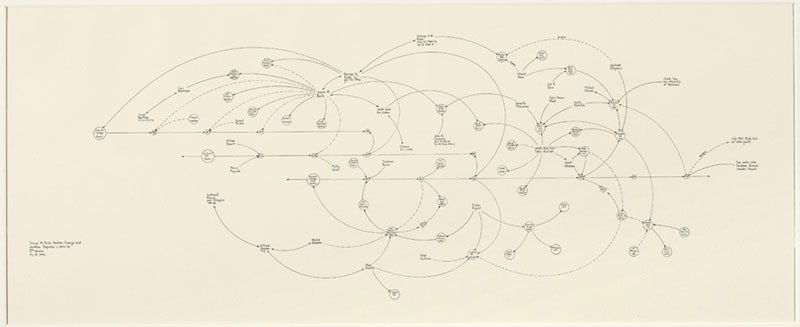
\includegraphics[width=0.8\linewidth]{includegraphics/Introduction_Lombardi-example}
	\end{subfigure}
\caption{Work of Mark Lombardi \cite{lombardi_ex}}\label{im:lombardi_ex}
\end{figure}
\textit{Orthogonal drawings} arise among others in VLSI design where quite many cables are following a similar path. The smallest angle between axis-aligned line segment is at most $\pi/2$ and their angular resolution is quite pleasing for the eye of the viewer. One fundamental, reliable model is the \textit{Kandinsky model} which is based on a \textit{grid embedding}. The vertices lie on a \textit{coarse} grid while the edges lie on a \textit{fine} grid extending the coarse grid. It may appear that an orthogonal drawing may convey some structural information, so \textit{smoothening} those edges is of interest. In this thesis, we focus on the smoothening of Kandinsky drawings by introducing circular arcs, inspired by \textit{Lombardi drawings} as illustrated in Figure \ref{im:lombardi_ex}\cite{lombardi_src1}\cite{lombardi_src2}. 
\begin{figure}[H]
	\centering
	\begin{subfigure}{0.45\textwidth}
		\centering
		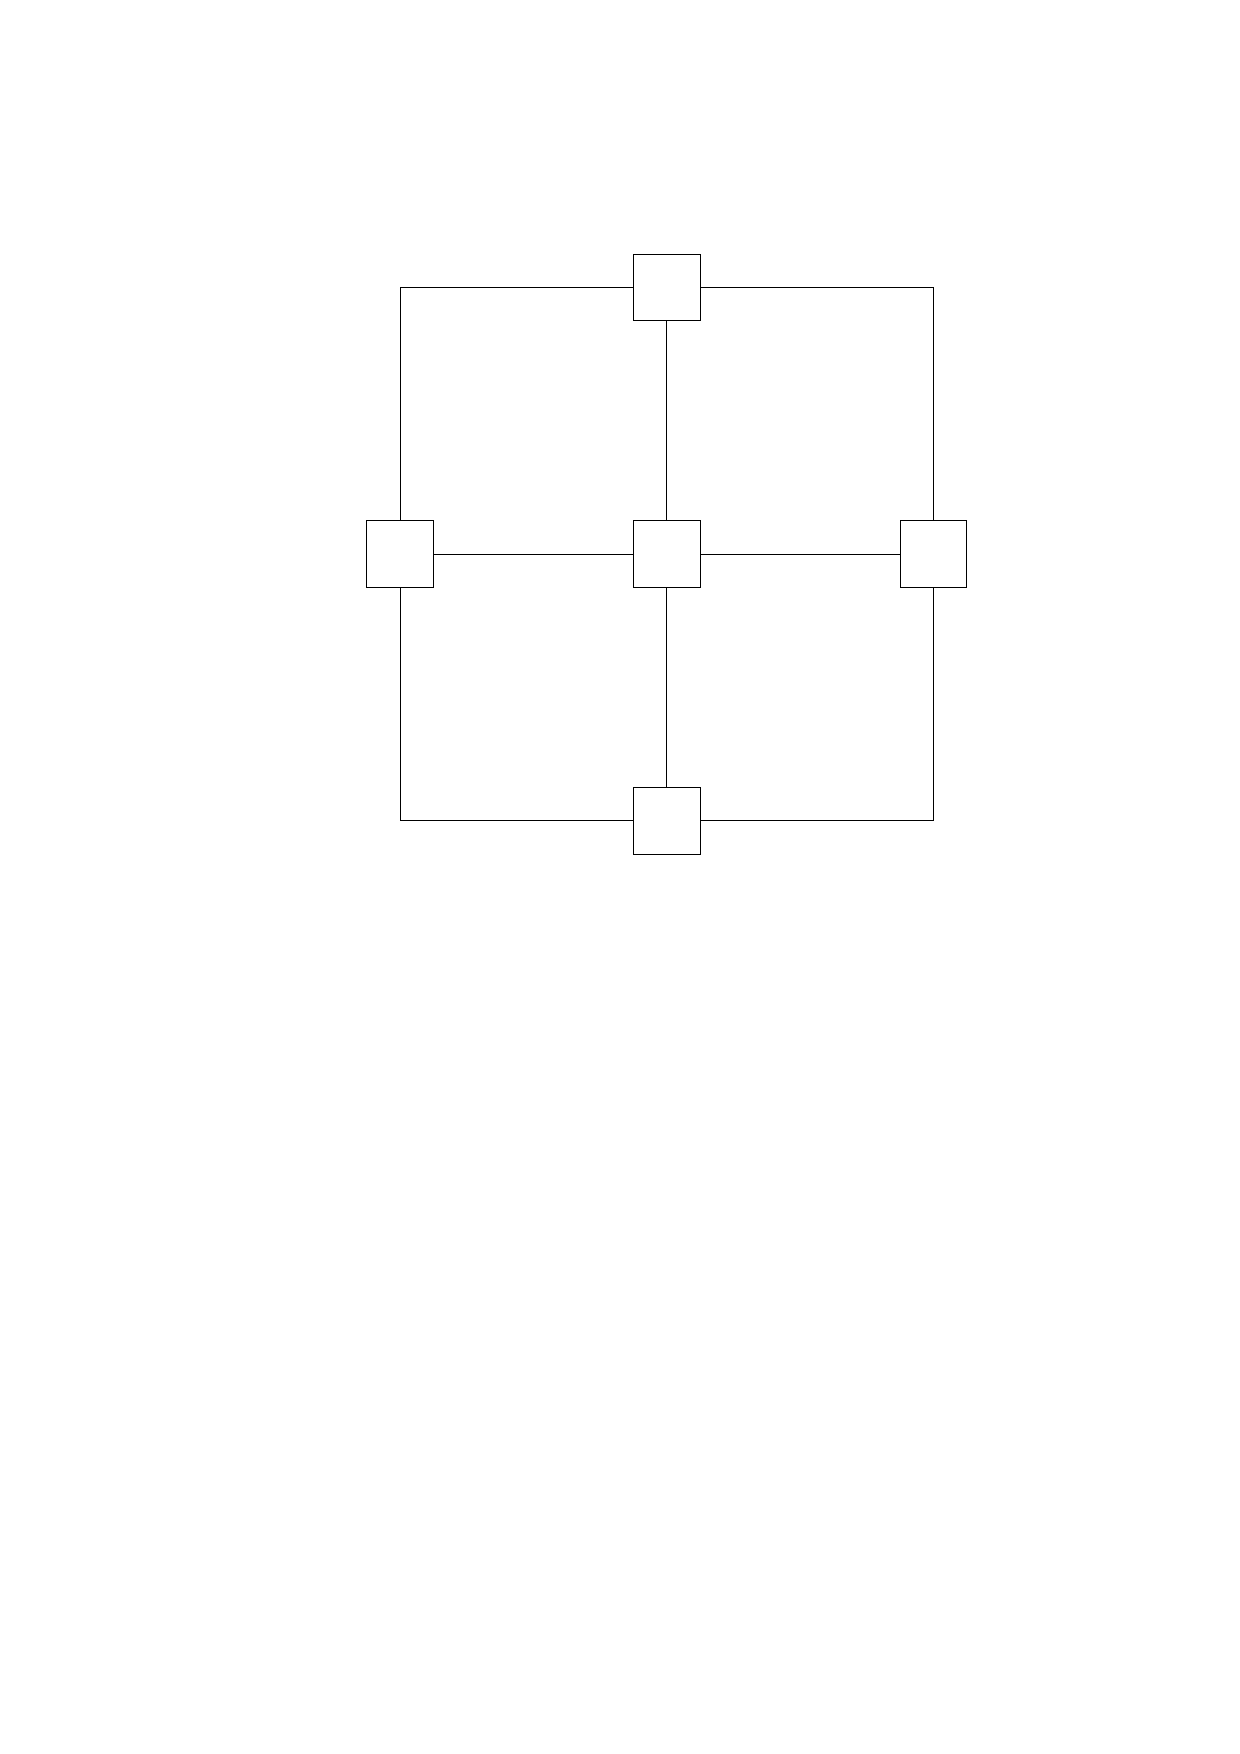
\includegraphics[width=0.4\linewidth,page=1]{includegraphics/introduction-example}
		\caption{Orthogonal drawing}\label{im:introduction_ex1}
	\end{subfigure}
	\begin{subfigure}{0.45\textwidth}
		\centering
		\includegraphics[width=0.4\linewidth,page=2]{includegraphics/introduction-example}
		\caption{Smoothened drawing}\label{im:introduction_ex2}
	\end{subfigure}
	\caption{Smoothening a drawing for aesthetic appeal}
\end{figure}
By postprocessing an input drawing like illustrated in Figure \ref{im:introduction_ex1} and \ref{im:introduction_ex2}, we also have to consider possible shape alternations. It is desirable that the orientation of the vertices is preserved, meaning that e.g. a metro map can still be read reasonably after the smoothening process\cite{metro1}.\\
However, it is a priori not guaranteed that there is a smoothening for every input Kandinsky drawing with a reasonable complexity increase. The introduction of circular arcs might arise some conflicts in sense of planarity. Dealing with postprocessing algorithms, we have to focus on new area bounds and the behaviour of the edge complexity in order to quantify the resulting quality of the smoothened drawing.
\label{key}\section{Preliminaries}
There are a variety of results regarding a special class of graphs - In the following section, let $G$ be a planar graph with maximum degree 4 and a port constraint. Every vertex is connected to at most one polyedge on each cardinal direction (North, South, East, West). 
\subsection{Fixed Layout Model}
Considering a drawing of an orthogonal graph $\Gamma_G$ in the Fixed Layout Model, the position of the vertices cannot be altered. This is a rather strict constraint. The implementation of circular arcs in a polyline lead to an increase of the edge complexity. Every bend is substituted with a quarter arc, resulting in two new bends in the worst case.
\begin{theorem}
	In the Fixed Layout Model, the edge complexity of a given orthogonal graph $G$ might increase from $k$ to $2k-1$.
\end{theorem}
The reason for the edge complexity increase is the fixation of the vertices and following counterexample regarding so-called \grqq Staircase Edges\grqq.
\begin{center}
	TODO: Staircase of 4-planar graph in Fixed Layout
\end{center}
It is already clear, that the Fixed Layout Model is rather too restrictive to process orthogonal graphs to SMOGs. A different approach is the Fixed Shape Model, where the embedding is contained regarding the circular ordering of the polyedges around a vertex.
\subsection{Fixed Shape Model}
In the Fixed Shape Model, the orientation of the vertices (North, East, West, South) and the embedding (circular ordering of the edges connected tp 1a vertex) is preserved. The vertices are of uniform size but can be repositioned on the course integer grid. Due to the horizontal stretching technique by the factor of $l$ (longest vertical segment), there is new space left and right from every vertical line segment. To be more precise, there is an empty box left and right from every vertical line with size $l'\times l'$, while $l'$ is the length of the regarding vertical line.\\
In practice, the SMOG Model is derived from the Kandinsky Model using basically two plane sweeps: The first plane sweep stretches the Kandinsky drawing horizontally by the factor of the longest vertical line segment. The second plane sweep erases 90 degree bends by circular arc substitution, making the drawing \textit{smooth}. The resulting drawing is in $\Rho(n^2) \times \Rho(n)$ area due to the horizontal stretching.
\begin{theorem}
	If the bends of a polyline are purely \underline{uniform} (in the same direction), then there is a SMOG representation of that polyline without an increase of complexity. Similarily, if the polyline is purely \underline{alternating}, the edge complexity raises from $k$ to $\lceil\frac{3}{2}k\rceil$.
\end{theorem}
\begin{sketch}
	If a polyline is purely uniform, consider the vertical segments; If the a vertical segment lies between two horizonal segments, substitute that vertical segment with a semicircle arc. If a vertical segment is connected to a vertex and a segment, substitute the vertical segment with a quadrant arc. If the polyedge consists of one vertical segment, then two vertices are at both ends. The edge is not altered. The space around a vertical segment, necessary for the circle arc substitution, is guaranteed by stretching the entire drawing horizontally by a factor of the longest vertical segment.
\end{sketch}
\begin{theorem}
	Let $G$ be an orthogonal graph. If any polyline is alternating at some point, $G$ can be minimized regarding the number of bends. \label{th:alt_not_min}
\end{theorem}
\begin{sketch}
	We show the theorem by flow minimization over the dual graph the following way: for each alternation we send one unit of flow from one face to another. Determining the unit of the minimized flow and the direction between both faces determines the minimal direction changes of an edge resulting in a lower number of bends.
\end{sketch}
\begin{theorem}
	In the Fixed Shape Model, an orthogonal graph $G$ - with minimal number of bends and an edge complexity of $k$ - can be transferred to a SMOG without an edge complexity increase under $\Rho(n^2) \times \Rho(n)$ area.
\end{theorem}
\begin{sketch}
	If $G$ has got a minimal number of bends, then there is no alternation in any polyline by contraposition of Theorem \ref{th:alt_not_min}. The polyedges are purely uniform and every vertical segment is replaced by either a quarter circle arc or a semicircle arc or it stays the same. As we already saw, uniform bends do not lead to an edge complexity increase. Planarity is preserved due to the stretching technique.
\end{sketch}
\section{The Kandinsky Model}
\subsection{Introduction}
Previous results show that the Fixed Shape Model is flexible in its methods to create the smooth orthogonal drawings deriving from orthogonal planar drawings with maximum degree four. The Kandinsky Model is a well-established model to create an orthogonal drawing of a graph of arbitrary degree with a reasonable edge complexity. However, the Kandinsky Model differs in its properties. The vertices lie on a coarse grid and are illustrated with uniform boxes. If multiple edges are connected to the same port, then at most one is connected to another vertex. 
\begin{definition}
	The \textit{bend or end} property of an orthogonal drawing of a graph means that from every polyedge connected to a specific port of a vertex at most one is connected to another vertex with an edge complexity of one. The remaining polyedges are at least of complexity two and bend in some point.
\end{definition}
It is to examine if postprocessing Kandinsky drawings guarantees the area required for circular arc substitution and whether or not the planarity of a drawing is preserved in any case. Furthermore, we will examine the edge complexity of SMOGs derived from Kandinsky drawings. We will see, that the edge complexity of any polyedge does not increase excessively.
\subsection{Area Investigation}
The idea of the stretching technique is to create new space between edges and vertices. By doing so, the space for circular arcs will be guaranteed. As we already saw, the stretching technique is sufficient for 4-planar graph drawings. But what about planar drawings of arbitrary degree?\\
There are two major cases to distinguish - either a vertical line segment is between two other segments or it is connected to a vertex therefore on one of the ends of the polyedge.
\subsubsection*{Between two segments - \grqq Boxing\grqq}
The stretching technique is a modification of an input graph fulfilling properties of the Fixed Shape Model. In this section we will examine the resulting space along vertical line segments. We will see that the new space created can be described as squares or \textit{1}~and we will see that the stretching technique will result in new space left and right from it.
\begin{lemma}
	Let $l$ be the longest vertical line segment in a given orthogonal drawing of a graph $G$. Then, after applying the stretching technique by the factor of $|l|$, every vertical line segment $l'$ which is between two segments got a new \grqq box\grqq~of space left and right from it of size $|l'|\times |l| \leq |l|^2$.\label{lem:space_stretch}
\end{lemma}
\begin{proof}
	Let $l'$ be a vertical line segment between two horizontal line segments. Then, by planarity of the orthogonal drawing, consider without loss of generality the minimum distance between $l'$ and another vertical line segment $l''$ by $\delta(l',l'') \geq 1$ on the fine integer grid. Stretching every horizontal line segment by adding a segment of size $|l|$ results in a stretching of the distance of two vertical line segments. The distance of vertical line segments can be considered as a horizontal subtraction. $$\delta(l',l'') = |l'_x - l''_x|$$
Stretching horizontally modifies the position of objects in x-coordinates only.
\begin{align}
\delta'(l',l'') = &|\left(|l| + |l'_x|) - (|l| + |l''_x|\right)|\\
 \underbrace{=}_{|l| > 0} &|l| + \left(|l'_x - l''_x|\right) = |l| + \delta(l',l'')
\end{align}
So the distance between a vertical line and an object increased to minimum $|l|+1$.
\end{proof}
\begin{figure}[H]
	\centering
	\begin{subfigure}{0.3\textwidth}
			\centering
			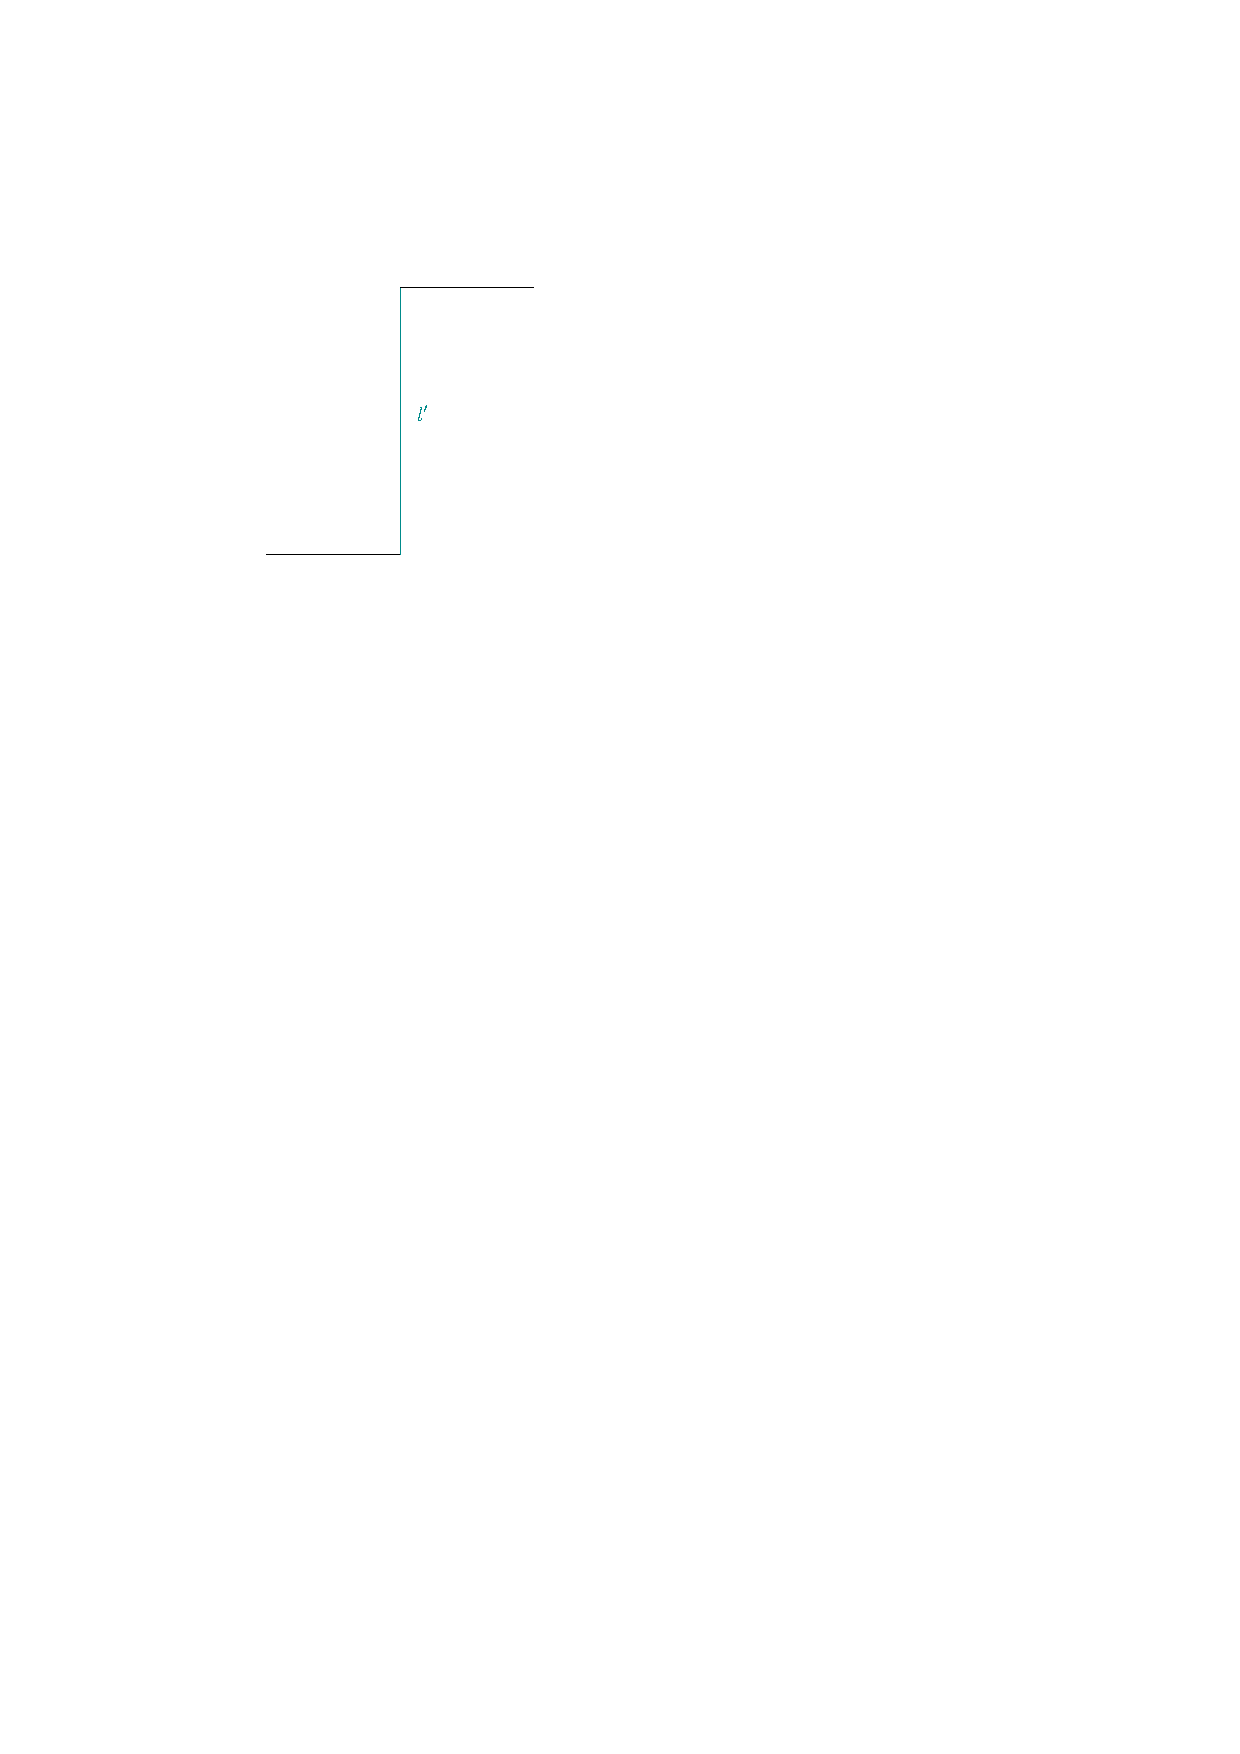
\includegraphics[width=0.7\linewidth,page=1]{includegraphics/boxing_alt.pdf}
			\caption{Orthogonal input edge}
	\end{subfigure}
	\begin{subfigure}{0.66\textwidth}
			\centering
			\includegraphics[width=0.7\linewidth,page=2]{includegraphics/boxing_alt.pdf}
			\caption{Two circular arcs result in +1 bend}\label{im:boxes}
\end{subfigure}
	\caption{The $l'\times l'$ box left and right from the original vertical line is empty after applying the stretching technique}
\end{figure}
This implies that there is new space to the left and right of a vertical line $l'$ between two segments of size $|l'|\times|l'|$. We will consider the new space as a free \grqq box\grqq~(Figure \ref{im:boxes}). This means that the space for different situations of SMOG substitution is guaranteed in the intermediate case.
\begin{lemma}
Let $l'$ be the vertical line intermediate in a fragment. Then, take the box of the corresponding side and draw a half circle segment with radius $r = \frac{l'}{2}$. Furthermore, the complexity does increase if and only if the fragment is alternating.
\end{lemma}
\begin{proof}
	Let $l'$ be the vertical line intermediate in a fragment after application of the stretching technique. Then, take the box of size $|l'| \times |l'|$ and center it around $l'$. Draw two quarter circle segment with the same radii $r = \frac{l'}{2}$ along the alternation. The area necessary is already guaranteed, all left to examine is the complexity increase in the alternating case which takes two bends away (get rid of the vertical line) and substitute with two quarter circle segments which result in three new bends. In the uniform case the complexity does not increase.
\end{proof}
\subsubsection*{Connected to a vertex}
If a vertical segment is connected to a vertex, then the boxing argument does not apply, since the space between multiple ports on the same side of a vertex is not altered by the stretching technique. We will see that this will not lead to a problem.
\begin{lemma}
	Let $\Gamma_G$ be any orthogonal Kandinsky drawing and $v \in V_G$ a vertex with its ports. Then, there is at most one edge connected to each port of $v$ with only one edge segment (complexity = 1). This describes the \textit{bend or end} property of the polyedges regarding a single port.\label{lem:bend_or_end}
\end{lemma}
\begin{proof}
	The vertices inherit a uniform size and are centered on a grid point. Either, a vertex is connected to another vertex with a single segment, then the center of both vertices share either the same $x$ or the $y$ coordinate, or two vertices are connected with a polyedge, then it has to bend at some point. The bend or end property of Kandinsky graphs is implied by the coarse grid on which the vertices are positioned. 
\end{proof}
So, regarding a port of a vertex $v$, the edges either bend or end in a vertex. Now we want to examine the area regarding the circular arcs of the SMOG model.
\begin{lemma}
	Consider a vertex $v$ and $p$ edges connected to a port. Then, in SMOG, at most one of the $p$ edges consists of a single segment ending in a vertex (as in Kandinsky). The other minimal $p-1$ edges start off with a circular arc, the original bend wanders along the horizontal segment and - most importantly - the complexity does not increase.\label{lem:Kandinsky_bend}
\end{lemma}
\begin{proof}
	The edge consisting of a single segment is not altered if it is vertical. If it is horizonal, the stretching technique adds the length of the longest segment. Therefore it does not change in its characteristics, only in length.\\
	Consider the other minimal $p-1$ edges which are bending in some point (Figure \ref{im:1vme1}).\\
	\begin{figure}[H]
		\centering
		\begin{subfigure}{0.3\textwidth}
			\centering
			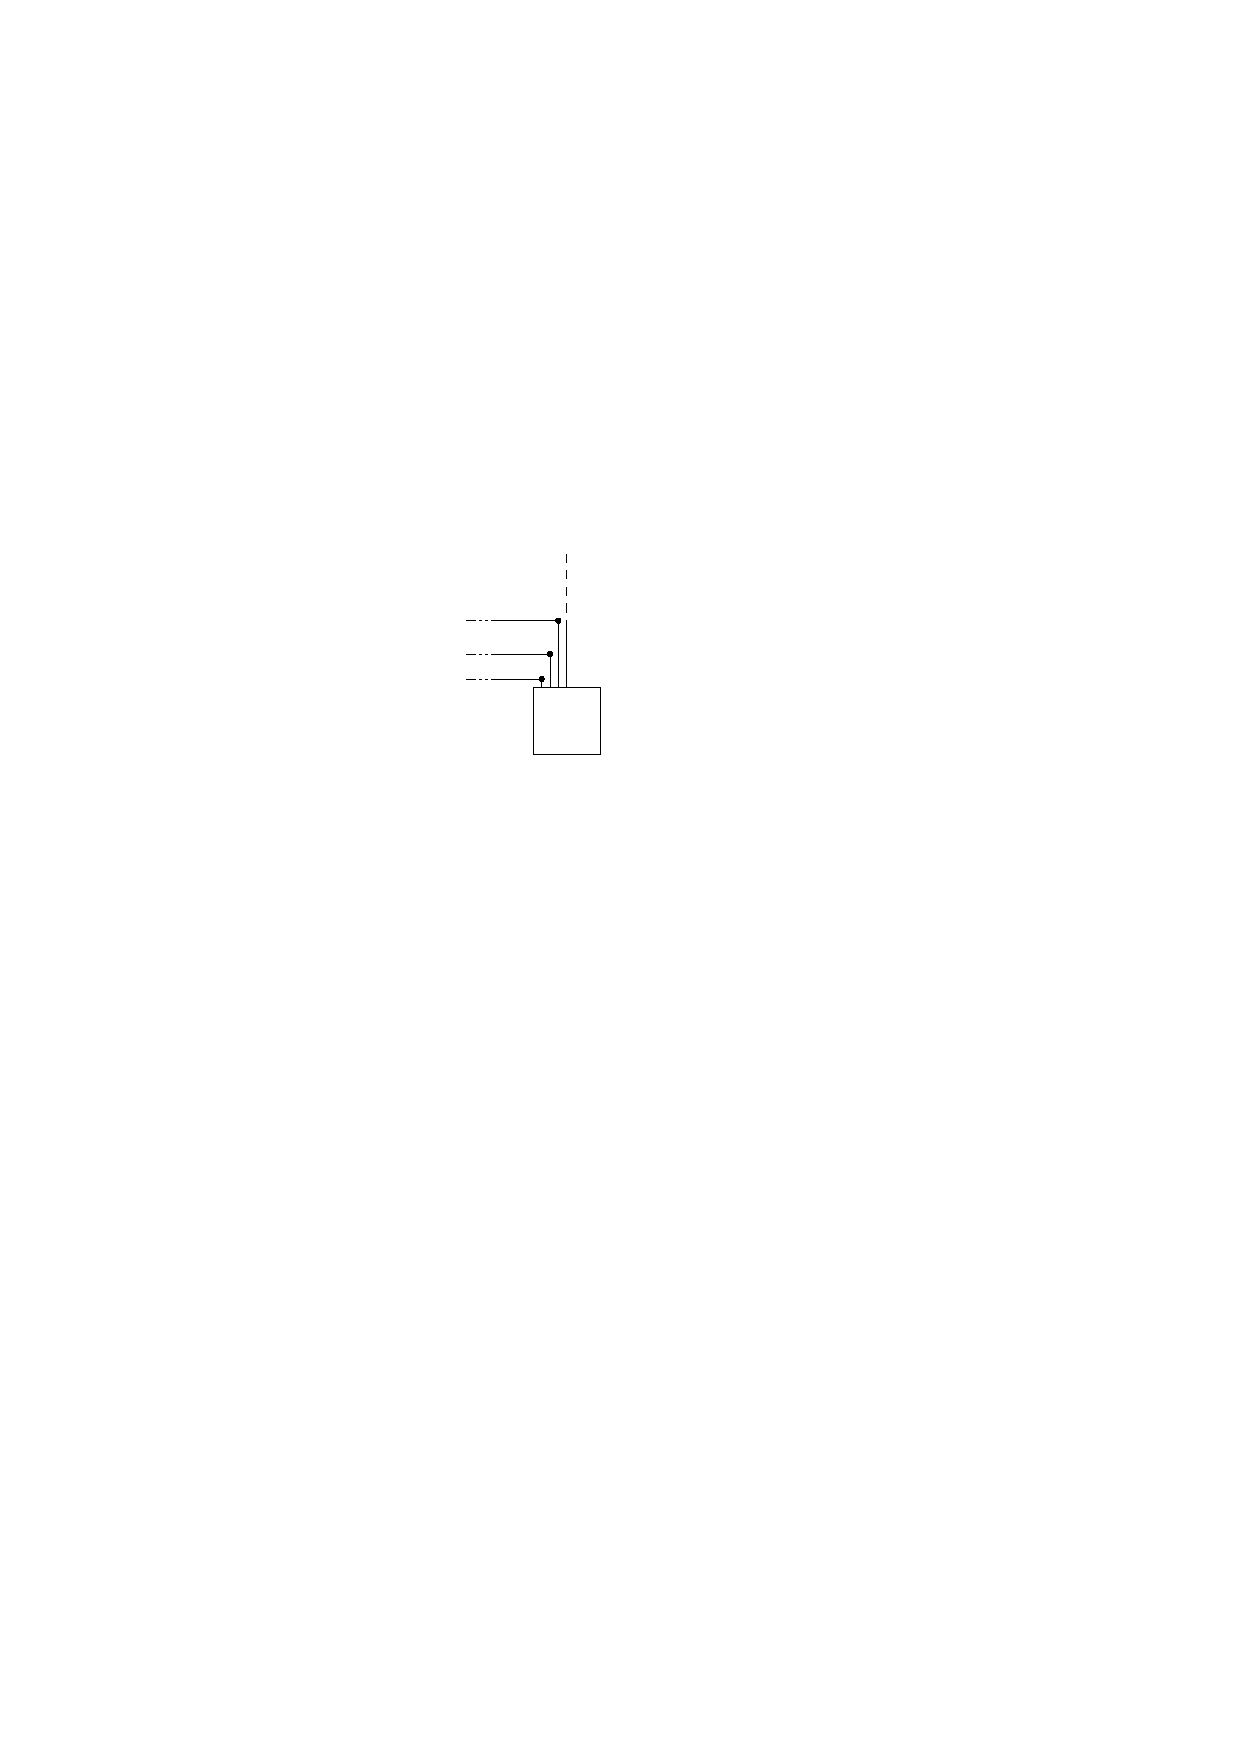
\includegraphics[width=0.55\linewidth,page=1]{includegraphics/1vertex-multEdges.pdf}
			\caption{Kandinsky situation}\label{im:1vme1}
		\end{subfigure}
	    \begin{subfigure}{0.3\textwidth}
		    \centering
		    \includegraphics[width=0.75\linewidth,page=2]{includegraphics/1vertex-multEdges.pdf}
		    \caption{}\label{im:1vme2}
	    \end{subfigure}
        \begin{subfigure}{0.3\textwidth}
	        \centering
	        \includegraphics[width=0.76\linewidth,page=3]{includegraphics/1vertex-multEdges.pdf}
	        \caption{SMOG representation}\label{im:1vme3}
        \end{subfigure}
        \caption{Smoothen multiple polyedges on the same port}\label{im:1vme}
	\end{figure}
The polyedges are connected equidistantly to a port. The increasing radii from outside-in (Figure \ref{im:1vme2}) and the original planarity in Kandinsky guarantee the planarity preservation of the resulting SMOG representation (Figure \ref{im:1vme3}).
\end{proof}
These results regarding graphs with arbitrary degree imply the functionality of the stretching technique even for the Kandinsky model. \cite[p. 582, Section 4.1]{SMOG}
\begin{corollary}
	Let $G$ be a graph with arbitrary degree and $\Gamma_G$ a planar orthogonal drawing in the Kandinsky model. Then, the stretching technique from \cite[p. 582, Section 4.1]{SMOG} is applicable guaranteeing the circular arc substitution. To be more precise, $\Gamma_G$ can be postprocessed to a SMOG representation, taking $\Rho(n^2) \times \Rho(n)$ area.
\end{corollary}
\begin{proof}
	The \textit{bend or end} property from Lemma \ref{lem:bend_or_end} and the Kandinsky bends in SMOG from Lemma \ref{lem:Kandinsky_bend} guarantee the preservation of the planarity and the necessary space for the circular arc substitution is given, as we can see in Lemma \ref{lem:space_stretch}. The worst case example drawing in the 4-planar situation regarding horizontal area bounds also takes effect in the $k$-planar situation.
	\begin{figure}[H]
		\centering
		\begin{subfigure}{.4\textwidth}
			\centering
			\includegraphics[width=0.7\linewidth,page=3]{includegraphics/4-planar_worst_case.pdf}
			\caption{Original orthogonal graph}	
		\end{subfigure}
		\begin{subfigure}{.6\textwidth}
			\centering
			\includegraphics[width=0.9\linewidth,page=4]{includegraphics/4-planar_worst_case.pdf}
			\caption{After applying the stretching technique}
		\end{subfigure}
		\caption{Recall the worst case situation of Figure \ref{im:4-planar_worst_case}}
	\end{figure}
\end{proof}
\subsection{Edge Complexity Investigation}
%The input will we a drawing of a graph in the Kandinsky Model, which means that there are only vertical and horizontal line segments, vertices illustrated in squares of a uniform size. Vertices lie on a course integer grid, while the line segment lie on a fine grid. The course grid is embedded in the fine grid.$$\text{Grid}_{\text{vertices}} \subset \text{Grid}_{\text{edges}}$$ A polyedge is an edge consisting of multiple line segments. The end of a line segment is either connected to another line segment or to a vertex. It is possible that multiple polyedges are connected to the same port of a vertex.\\
As we saw in the previous section, the possibility of a SMOG representation is given even if the degree of the graph is arbitrary. All that remains is the examination regarding the number of bends of a polyedge. Previous results deliver an upper bound for $4$-planar graphs, a polyedge with complexity $k$ in the orthogonal drawing is bound by $\left\lfloor\frac{3}{2}\right\rfloor$ in the fixed shape model. We will see, that this upper bound still pertains.\\
Let $G$ be a planar graph with arbitrary degree, an orthogonal drawing $\Gamma_G$ is given and let $k$ describe the edge complexity of a polyedge of $\Gamma_G$. The main goal of this section is to examine lower and upper bounds for $k$ in SMOG.
%\begin{theorem}
%Let $\Gamma_G$ be an orthogonal drawing. Then: $$OC_{k+1} \hookrightarrow SC_{2k+1}$$ under the Fixed Layout Model.
%\end{theorem}
%\begin{proof}[Proof]
%Consider following graph:
%\begin{center}
%\texttt{TODO: Staircase graph}
%\end{center}
%As you can see, the upper bound is strict in this case due to the fix position of the vertices.
%\end{proof}
%\subsection{Fixed Shape Model}
%The only case where the new space is not guaranteed are vertical line segments ending in a vertex along with other vertical lines ending at the same port. We shall see that this will not be a problem regarding the edge complexity.\\
%In practice, the SMOG Model is derived from the Kandinsky Model using basically two plane sweeps: The first plane sweep stretches the Kandinsky drawing horizontally by the factor of the longest vertical line segment. The second plane sweep erases 90 degree bends by circular arc substitution, making the drawing \textit{smooth}. The resulting drawing is in $\Rho(n^2) \times \Rho(n)$ area due to the horizontal stretching.
\subsubsection*{Examining \grqq good\grqq~and \grqq bad\grqq~parts of a polyline}
The general idea is to distinguish between two major cases: Line segments with alternating turns (staircase, zig-zags) and line segments with uniform turns (spirals, u-shapes). As we already saw, the SMOG representation of uniform turns does not increase the edge complexity. Therefore we examine polyedges regarding its properties of turns from one vertex to another. We will try to maximize the uniform part and simultaneously minimize the alternating part of a polyedge. We achieve this by so-called \textit{fragmentation} of a polyedge.
\begin{definition}
	An \textit{edge fragment} is a non-empty sequence of line segments. A \textit{fragmentation} of a polyedge is a sequence of fragments.
\end{definition}
The main advantage of the fragmentation is that every fragment can be seen as an independent polyedge.
The property of turns is crucial for the edge complexity thus the main criterion for the fragmentation.
\begin{definition}
	Like in Definition \ref{def:uni_alt}, a fragment is uniform if and only if all turns share the same direction. A fragment is alternating if and only if the turns are all alternating. A fragment is valid if and only if its turn property is either alternating or uniform.
\end{definition}
\begin{lemma} The fragmentation of a given polyedge $e$ is not unique.
\end{lemma}
\begin{proof}
	Consider the polyedge $(1,2)$ illustrated at Figure \ref{im:nonunique}. Algorithm \ref{algo:frag} takes the first three segments, considers its turn property and iterates along the polyedge. In the first picture, the segments starting from vertex 1 are obviously alternating, resulting in an uniform fragment consisting of only one segment. Similarily, starting at vertex 2, the first three fragments are uniform, the rest along to vertex 1 alternating. Both fragmentations are correct.
	\begin{figure}[H]
		\centering
		\begin{subfigure}{0.4\textwidth}
			\centering
			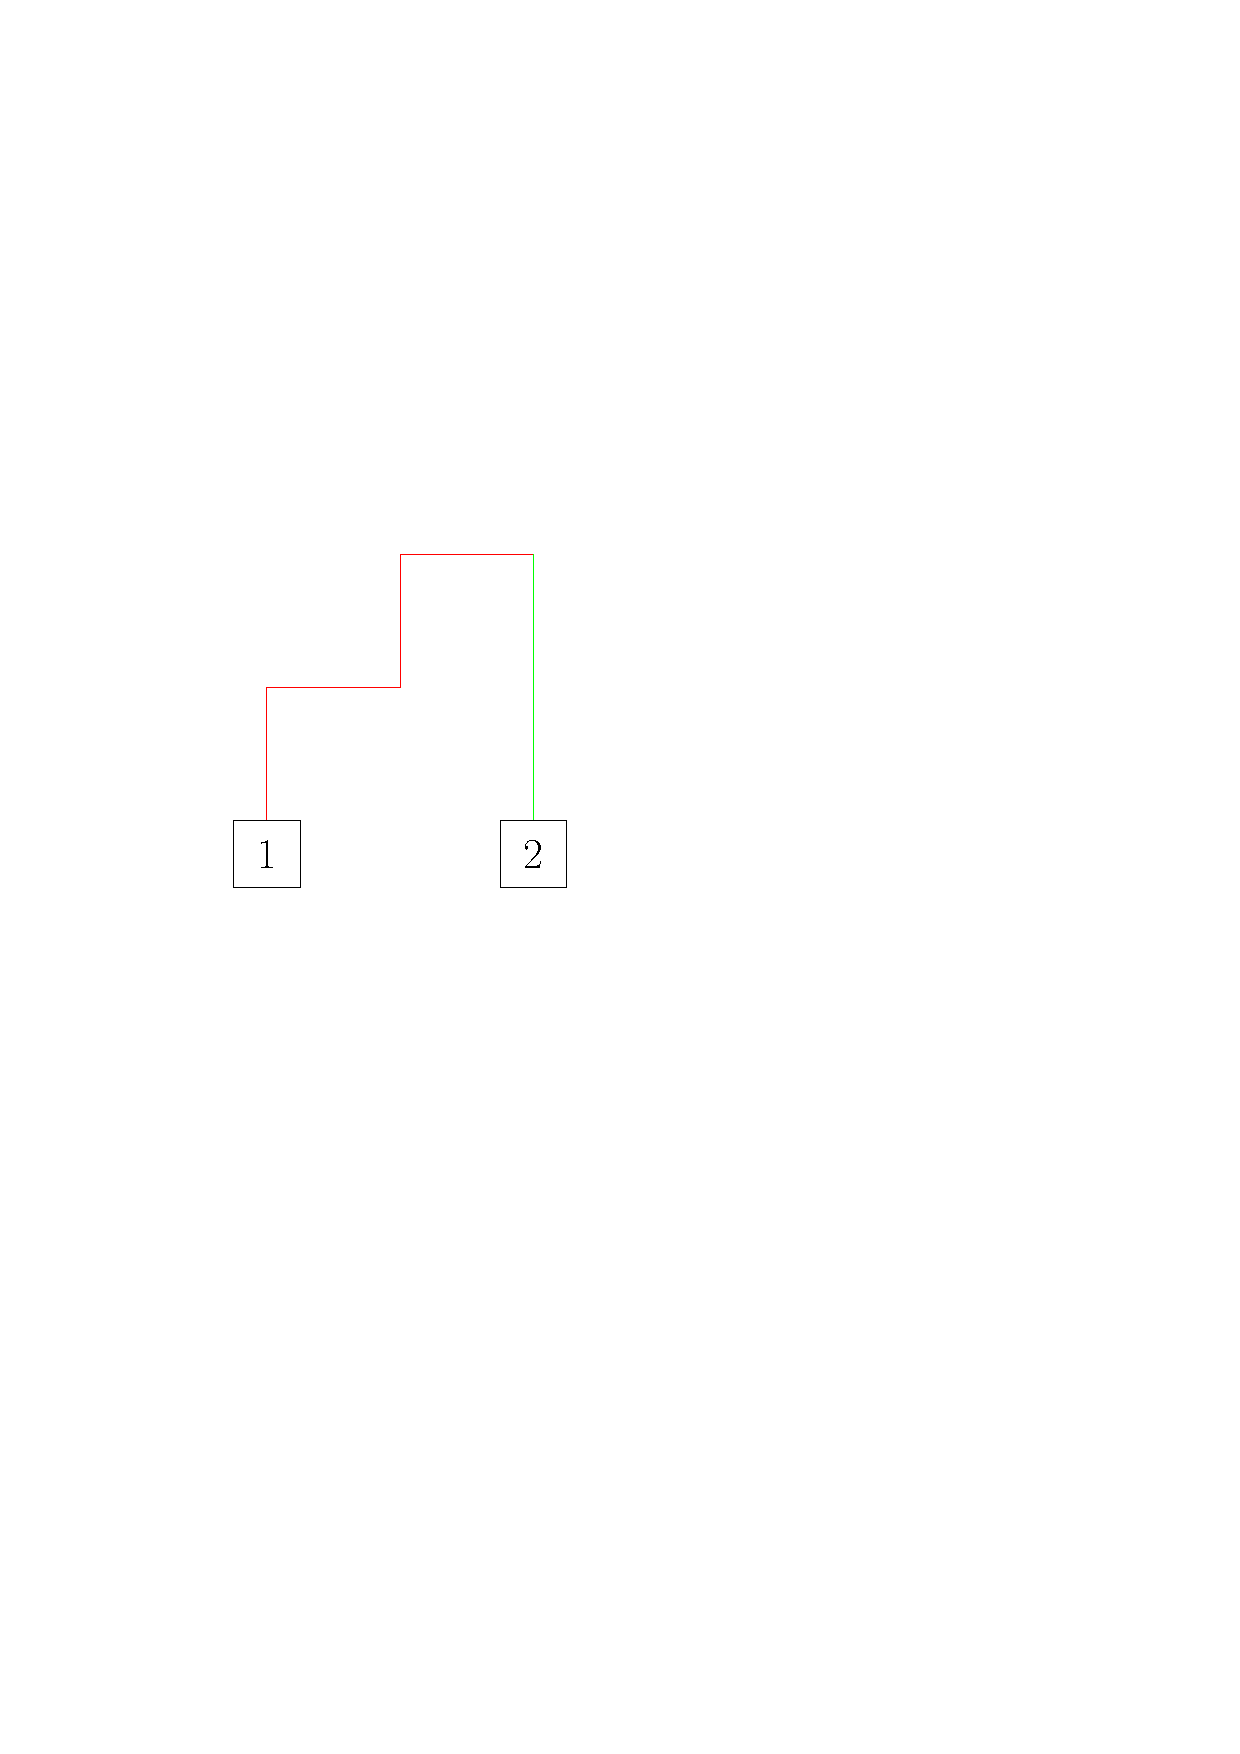
\includegraphics[width=0.6\linewidth,page=1]{includegraphics/non-unique-frag.pdf}
			\caption{Fragmented from $1$ to $2$}
		\end{subfigure}
		\begin{subfigure}{0.4\textwidth}
			\centering
			\includegraphics[width=0.6\linewidth,page=2]{includegraphics/non-unique-frag.pdf}
			\caption{Fragmented from $2$ to $1$}
		\end{subfigure}
		\caption{Non-unique fragmentation}\label{im:nonunique}
	\end{figure}
\end{proof}
\begin{definition}
	Let $e'$ and $f'$ be two fragmentations. Then 
	\begin{align*}e' \thicksim_R f' \Leftrightarrow \Gamma_{e'} = \Gamma_{f'}
	\end{align*}\label{def:frag_relation}
\end{definition}
This means that two fragmentations are relative if and only if they describe the same polyedge in a given drawing.
\begin{lemma}
	The relation from Definition \ref{def:frag_relation} is an equivalence relation.
\end{lemma}
\begin{proof}
	Describing the same image is trivially reflexive, symmetical and transitive.
\end{proof}
\begin{definition}
	Two fragments $f$ and $g$ are called incompatible if any segment transfer between $f$ and $g$ result in a turn property collision (Figure \ref{im:incompatible}).
\end{definition}
\begin{figure}[h]
	\centering
	\begin{subfigure}{0.4\textwidth}
		\centering
		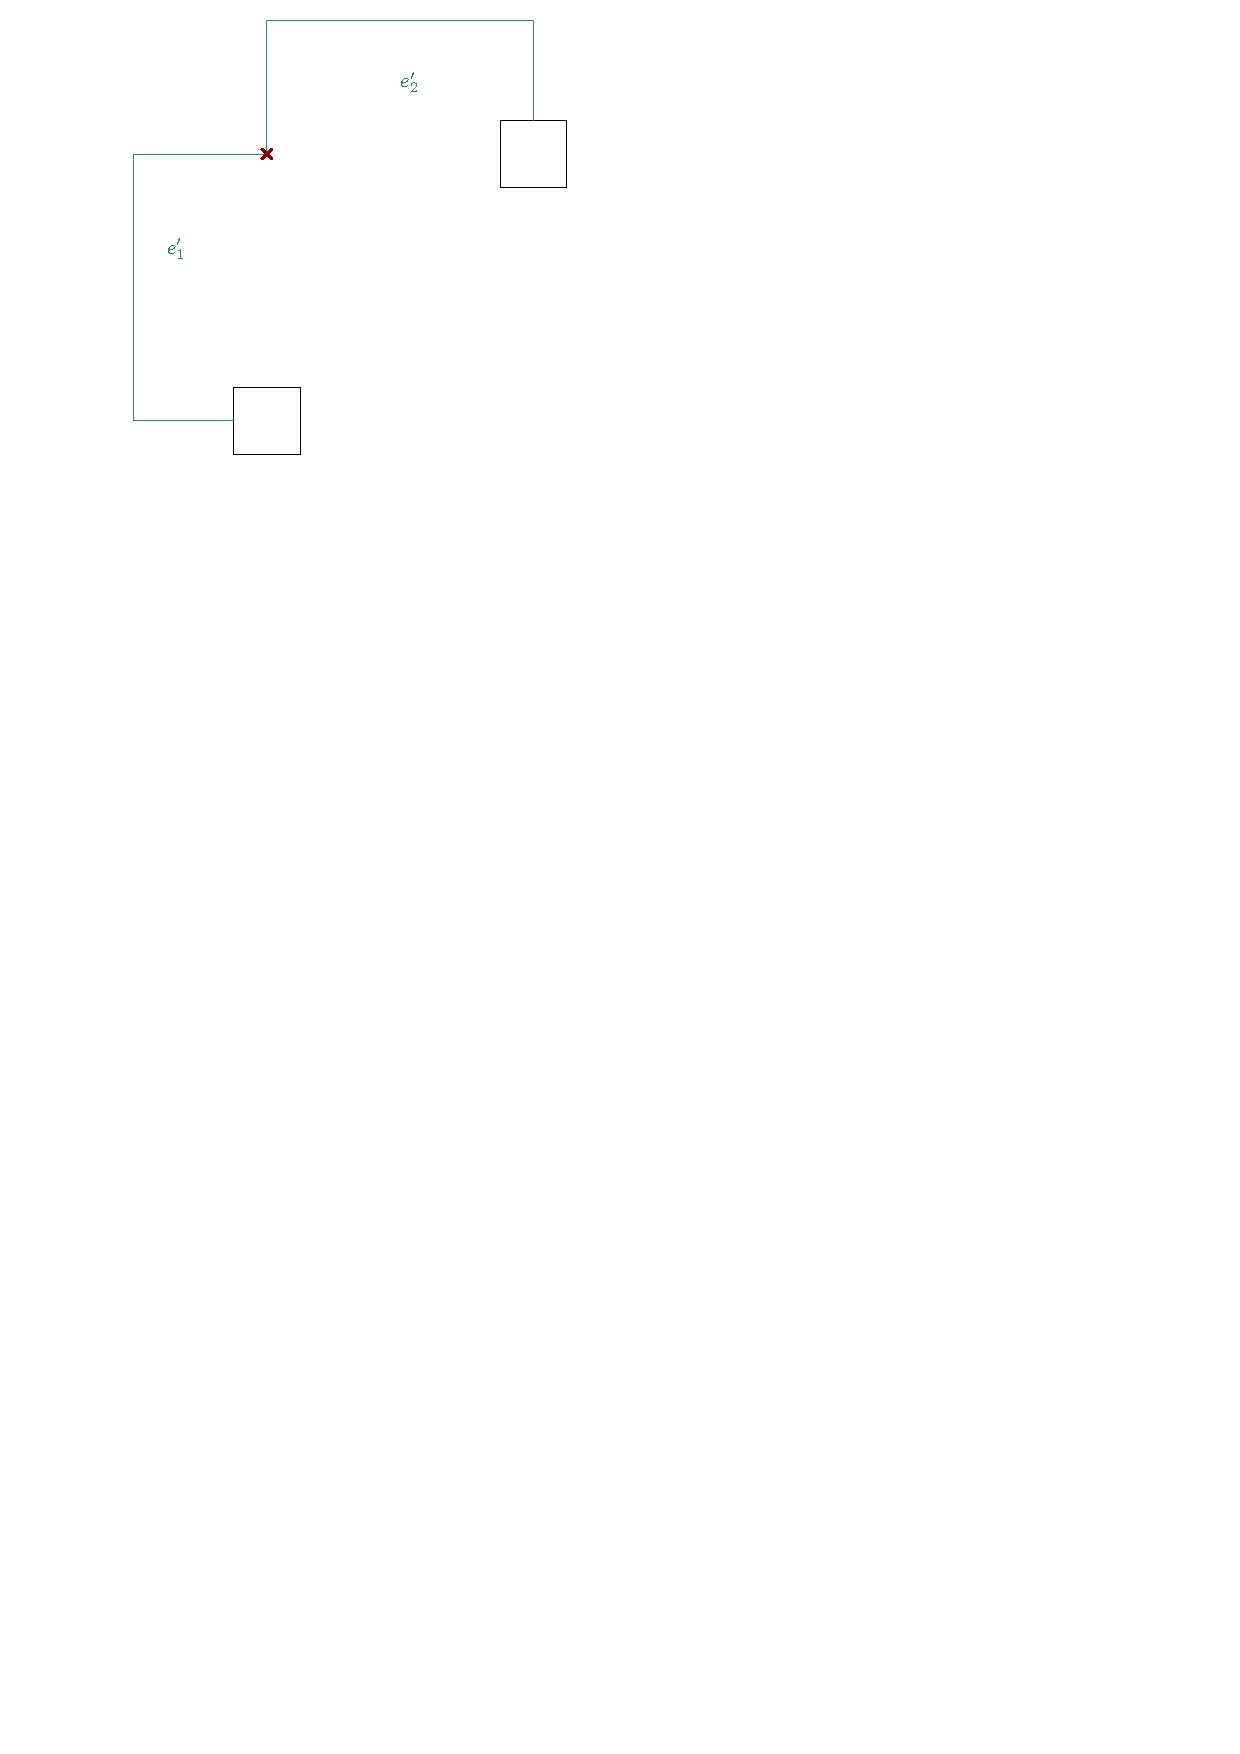
\includegraphics[width=0.7\linewidth,page=1]{includegraphics/unmergable_frags.pdf}
	\end{subfigure}
	\caption{Incompatible uniform fragments $e'_1,e'_2$}\label{im:incompatible}
\end{figure}
What if the polyedge we want to fragment inherits an edge complexity of at most 2? Fragmentation is meant to partition large polyedges but the case for $k\leq 2$ still has to be considered. Note, that fragments of length up to two are simultaneously uniform and alternating. For a definite statement, those fragments lack in the third segment
When we encounter a fragment of length two, we will interpret it as a uniform fragment first since uniformity does not necessarily increase the complexity. So now we are able to create a first - rather naive - algorithm in order to find a valid fragmentation.\newpage
\begin{algorithm}[H]
	\KwIn{Polyedge $e$ with edge complexity $k,k\geq 2$}
	\KwResult{$e'$, a first fragmentation of $e$}
	\If{$k = 2$}{
		$e'_1\gets (e_1,e_2)$\\
		$e'_1.\texttt{uniform = true}$\\
		$e' \gets (e'_1)$
	}
	\Else{
		$e'_1 \gets (e_1,e_2,e_3)$\\
		$e' \gets \emptyset$\\
		$i \gets 1$\\
		\If{$e'_1$ uniform}{$e'_1.\texttt{uniform} = \texttt{True}$}
		\Else{$e'_1.\texttt{uniform} = \texttt{False}$}
		\For{$j = 4$ to $k$}{
			\If{$e_j$ fits into the turn property of $e'_i$}{
				$e'_i.\texttt{append}$($e_j$)
			}
			\Else{
				%create a new fragment with $e'_m.\texttt{uniform} \gets \neg e'_{m-1}.\texttt{uniform}$ and continue
				$e'.\texttt{append}(e'_i)$\\
				$i \gets i + 1$\\
				$e_i.\texttt{uniform} = \neg e_{i-1}.\texttt{uniform}$\\
				$e_i \gets (e_j)$
			}
		}
	}
	$e'.\texttt{append}(e'_i)$\\
	\Return $e'$
	\caption{\texttt{fragment\_naively}$(e) \in \Rho(k)$}\label{algo:frag}
\end{algorithm}
\subsubsection*{Correctness of Algorithm \ref{algo:frag}}
This algorithm works for polyedges of length at least two. If the length is two, then the fragmentation will be unique since a fragment of length two is both uniform and alternating. If the complexity of the polyedge is greater than two, then lines 6 to 12 initialize the first fragment of length three and determines its turn property. For the remaining segments, this algorithm tests whether the next segment fits into the current fragment and appends it, if that is the case. If not, then the current fragment is appended to the returning fragmentation and a new fragment is created with the opposite turn property. By testing for every segment this algorithm returns a valid fragmentation and runs in $\Rho(k)$ by testing for every segment whether it would fit into the current fragment.
\\\\We will see in the following lemma, that this algorithm should be improved.
\begin{lemma}
	Algorithm \ref{algo:frag} is not sufficient to determine a satisfying fragmentation.
\end{lemma}
\begin{proof}
	Consider following polyedge given in Figure \ref{im:bad_frag}. By applying algorithm \ref{algo:frag}, we achieve the following fragmentation. Green fragments illustrate uniform ones, red ones illustrate alternating ones. Red dots illustrate the breaking point in the fragment creation.
	\\
	\begin{figure}[h]
		\centering
		\begin{subfigure}{0.3\textwidth}
			\centering
			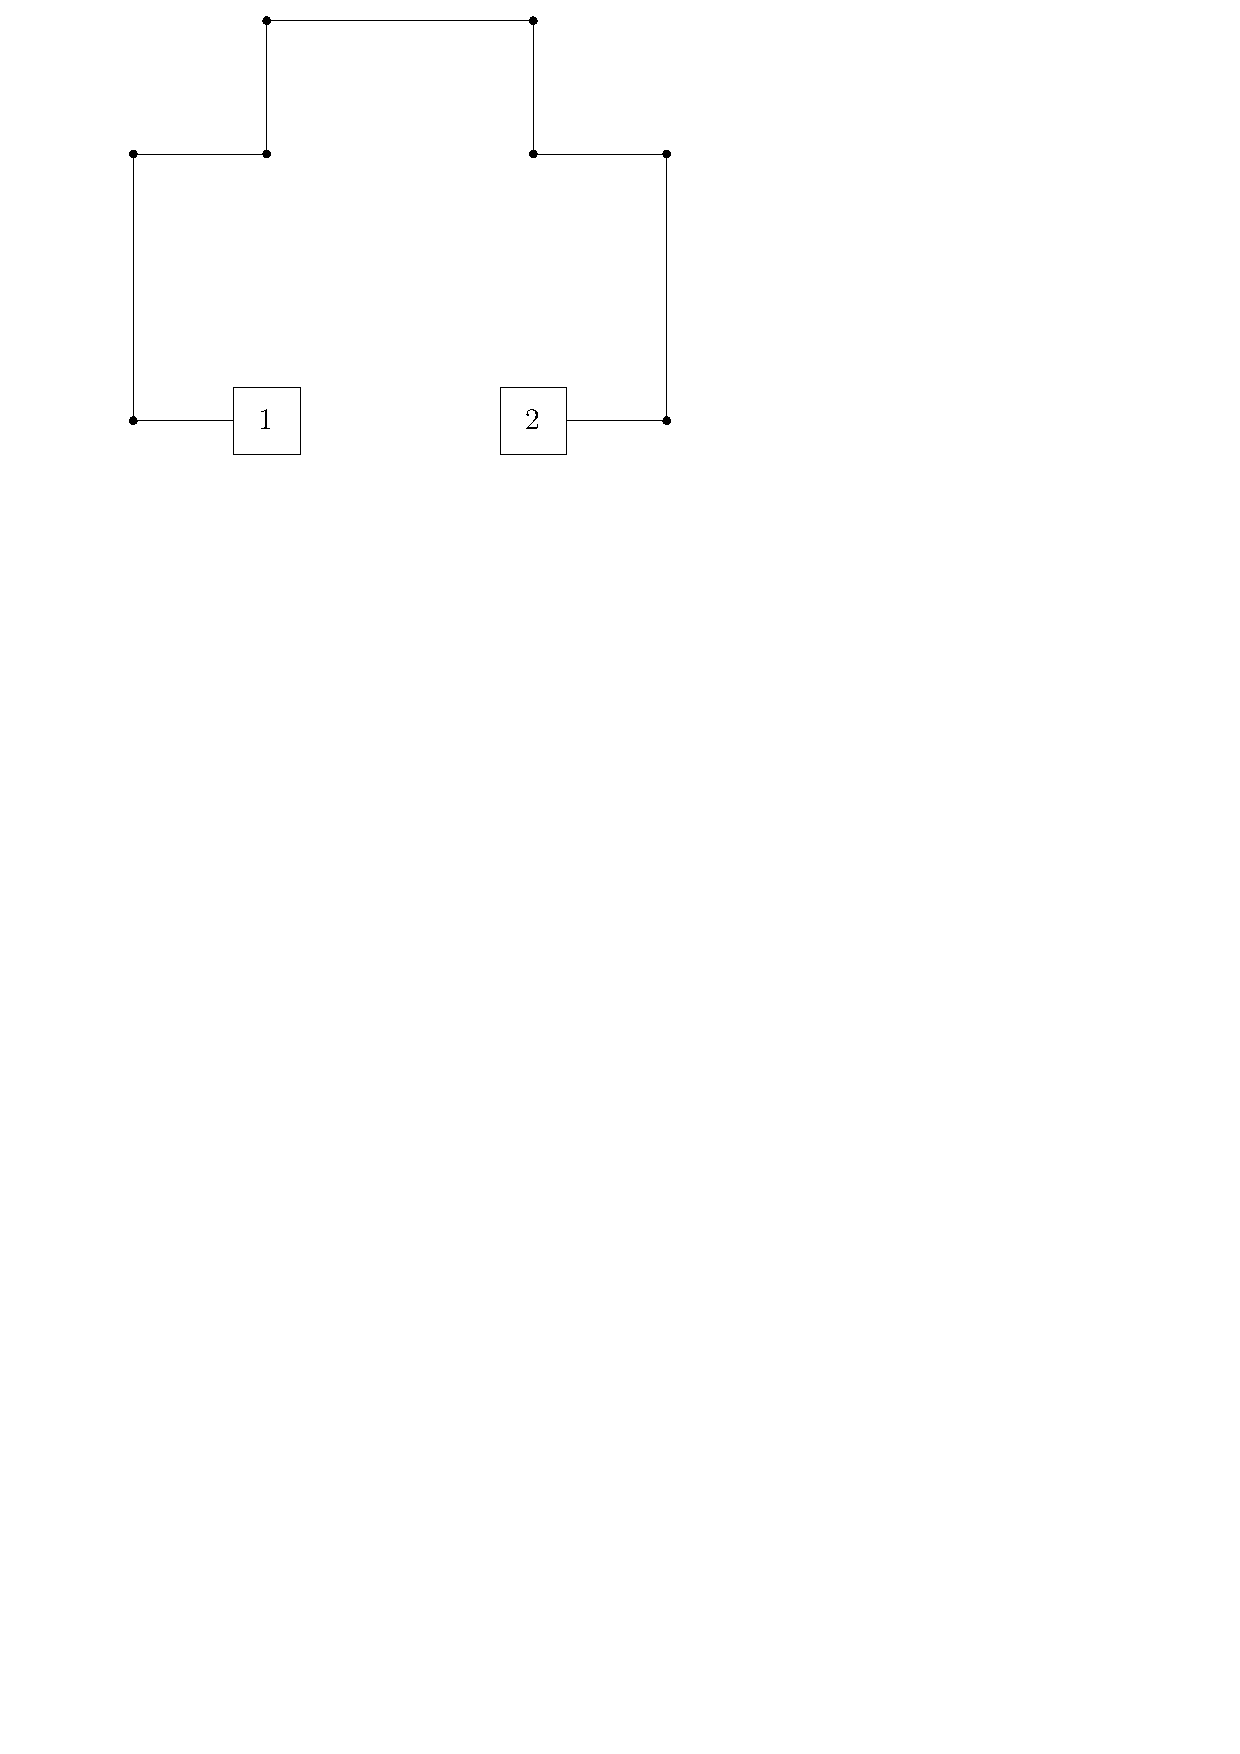
\includegraphics[width=0.7\linewidth,page=1]{includegraphics/bad_fragmentation.pdf}
			\caption{original input polyedge}\label{im:bad_frag1}
		\end{subfigure}
		\begin{subfigure}{0.3\textwidth}
			\centering
			\includegraphics[width=0.7\linewidth,page=2]{includegraphics/bad_fragmentation.pdf}
			
			\caption{Result of algorithm \ref{algo:frag}}\label{im:bad_frag2}
		\end{subfigure}
		\begin{subfigure}{0.3\textwidth}
			\centering
			\includegraphics[width=0.7\linewidth,page=3]{includegraphics/bad_fragmentation.pdf}
			
			\caption{more appreciating result}\label{im:bad_frag3}
		\end{subfigure}
		\caption{Bad example of a polyedge for algorithm \ref{algo:frag}}
		\label{im:bad_frag}
	\end{figure}
	\\
	As we can see in Figure \ref{im:bad_frag2}, algorithm \ref{algo:frag} delivers a fragmentation which consists of multiple fragments of length two. That is because algorithm \ref{algo:frag} forces two consecutive fragments to differ in their turn property. As we already know, fragments of length two are not that conclusive in this case. The result given in Figure \ref{im:bad_frag3} consists of longer fragments and seems to be somehow more precise regarding the polyedge. The big difference lies in the abortion of the change constraint regarding consecutive fragments.
\end{proof}
How do we find the best way to describe a polyedge as a fragmentation? One way to approach it is to minimize the total number of fragments and the number of alternating fragments.
\begin{lemma}
	The amount of all possible fragmentations of a polyedge $e$ is finite. To be more precise: $$|[e]_{\thicksim_R}| < 2^{k^2}$$
\end{lemma}
\begin{proof}
	Given a polyedge $e$, the amount of possible fragments $s$ is computed:
	\begin{align*}
	s &\leq \sum_{i=1}^k \frac{k}{i} \cdot i = k^2
	\end{align*}
	$i$ denotes the length of the fragments starting from $1$ to $k$. Consider $e$ partitioned into $\frac{k}{i}$ fragments, then there are $\leq i$ ways to start the fragmentation. The offset lies in $[0,i-1]$. The cardinality of the power set containing all possible fragments values $2^{k^2}$.
\end{proof}
As we already saw, there are multiple ways to describe a polyedge regarding a fragmentation. The next step is to determine, which fragmentation suits the best. Given a mathematical description to a given polyedge $e$, we want to describe the \grqq best way\grqq~to determine the number of bends in SMOG. So we will pick the \grqq best\grqq~fragmentation, which will be minimal in its number of alternating fragments and minimal in its total number of fragments. This leads to the following ordering relation:
\begin{definition}\label{def:ord_rel}
	Let $e',f'$ be two fragmentations of the same polyedge $e$ ($e' \thicksim_R f'$). Then we define the so-called \textit{FragOrder} relation:
	\begin{align*}
	e' \leq f' \Leftrightarrow \left(\#_{\text{altFrag}}(e') \leq \#_{\text{altFrag}}(f')\right) \wedge \left(\#_{\text{totalFrag}}(e') \leq \#_{\text{totalFrag}}(f')\right)
	\end{align*}
\end{definition}
\begin{lemma}
	\textit{FragOrder }is sufficient to determine a minimum of $[e]_{\thicksim_R}$. 
\end{lemma}
\begin{proof}
	Obviously, the relation $\leq$ is reflexive and transitive. Therefore, this relation is a preorder and we are able to determine a minimum of $[e]_{\thicksim_R}$ because in a finite set there is a minimum regarding a preorder.
\end{proof}
Comparing all possible fragmentations for the minimum will result in an exponential runtime. In order to fix this problem, we will take a slightly different approach - we will further get rid of alternating fragments by creating uniform-only fragments. This will result in longer fragmentations at first but we will see that it will be acceptable due to a new interpretation of this fragmentation.\\
We will be able to substitute alternating fragments as a sequence of uniform fragments.
\begin{lemma}
	A fragment $f$ of length $k'$ is alternating if and only if its purely uniform fragmentation $f'$ of size $\left\lceil\frac{k'}{2}\right\rceil$ inherits uniform incompatible fragments of length 2 and $f \thicksim_R f'$ regarding the FragOrder relation. This enables us to distinguish uniform fragments from alternating ones in the output of Algorithm \ref{algo:2ndfrag}.\label{lem:alt_2uni}
\end{lemma}
\begin{proof}
	If a fragment $f$ of length $k'$ is alternating, then every bend differs in its direction regarding the previous one. A fragment of length 2 inherits one bend. In an alternating fragment, the next one will cause a turn property collision, resulting in a new fragment. Again, fragments of lengths up to 2 are uniform by definition. Similarily, consider a sequence of fragments of length 2. If there were an optimization possible, then the sequence would not be completely incompatible as stated. This implies the staircase situation.
\end{proof}
We are willing to lengthen the fragmentation by coincidentally describing more precisely. This leads to a modification of algorithm \ref{algo:frag}.\\
\begin{algorithm}[H]
	\KwIn{Polyedge $e$ with edge complexity $k$,$k\geq 2$}
	\KwOut{Almost optimal fragmentation of $e$}
	$e'_1 \gets (e_1,e_2)$\\
	$f \gets \emptyset$\\
	$i \gets 1$\\
	\For{$j = 3$ to $k$}{
		\If{$e'_i.\texttt{append}(e_j)$ is uniform}{
			$e'_i.\texttt{append}(e_j)$
		}
		\Else{
			$f.\texttt{append}(e'_i)$\\
			$i \gets i+1$\\
			$e'_i\gets (e_j)$
		}
		
	}
	$f.append(e'_i)$\\
	\texttt{Recheck}$(f)$\label{algo:2ndfrag_recheck}\\
	\Return $f$
	\caption{\texttt{fragment\_uniform-only}$(e)$ $\in \Rho(k)$}\label{algo:2ndfrag}
\end{algorithm}
\subsubsection*{Correctness of algorithm \ref{algo:2ndfrag}}
This algorithm is pretty similar to algorithm \ref{algo:frag} with the big difference, that every fragment is now uniform. Initializing $f$ as a list of fragments, this algorithm appends the current fragment if the next segment collides with its turn property. Unless there is only one segment left in the end, every fragment consists of at least two segments. On the other side, there are optimal fragmentations which inherit a fragment of length one. Consider algorithm \ref{algo:2ndfrag} without line \ref{algo:2ndfrag_recheck}.
\begin{figure}[H]
	\centering
	\begin{subfigure}{0.3\textwidth}
		\centering
		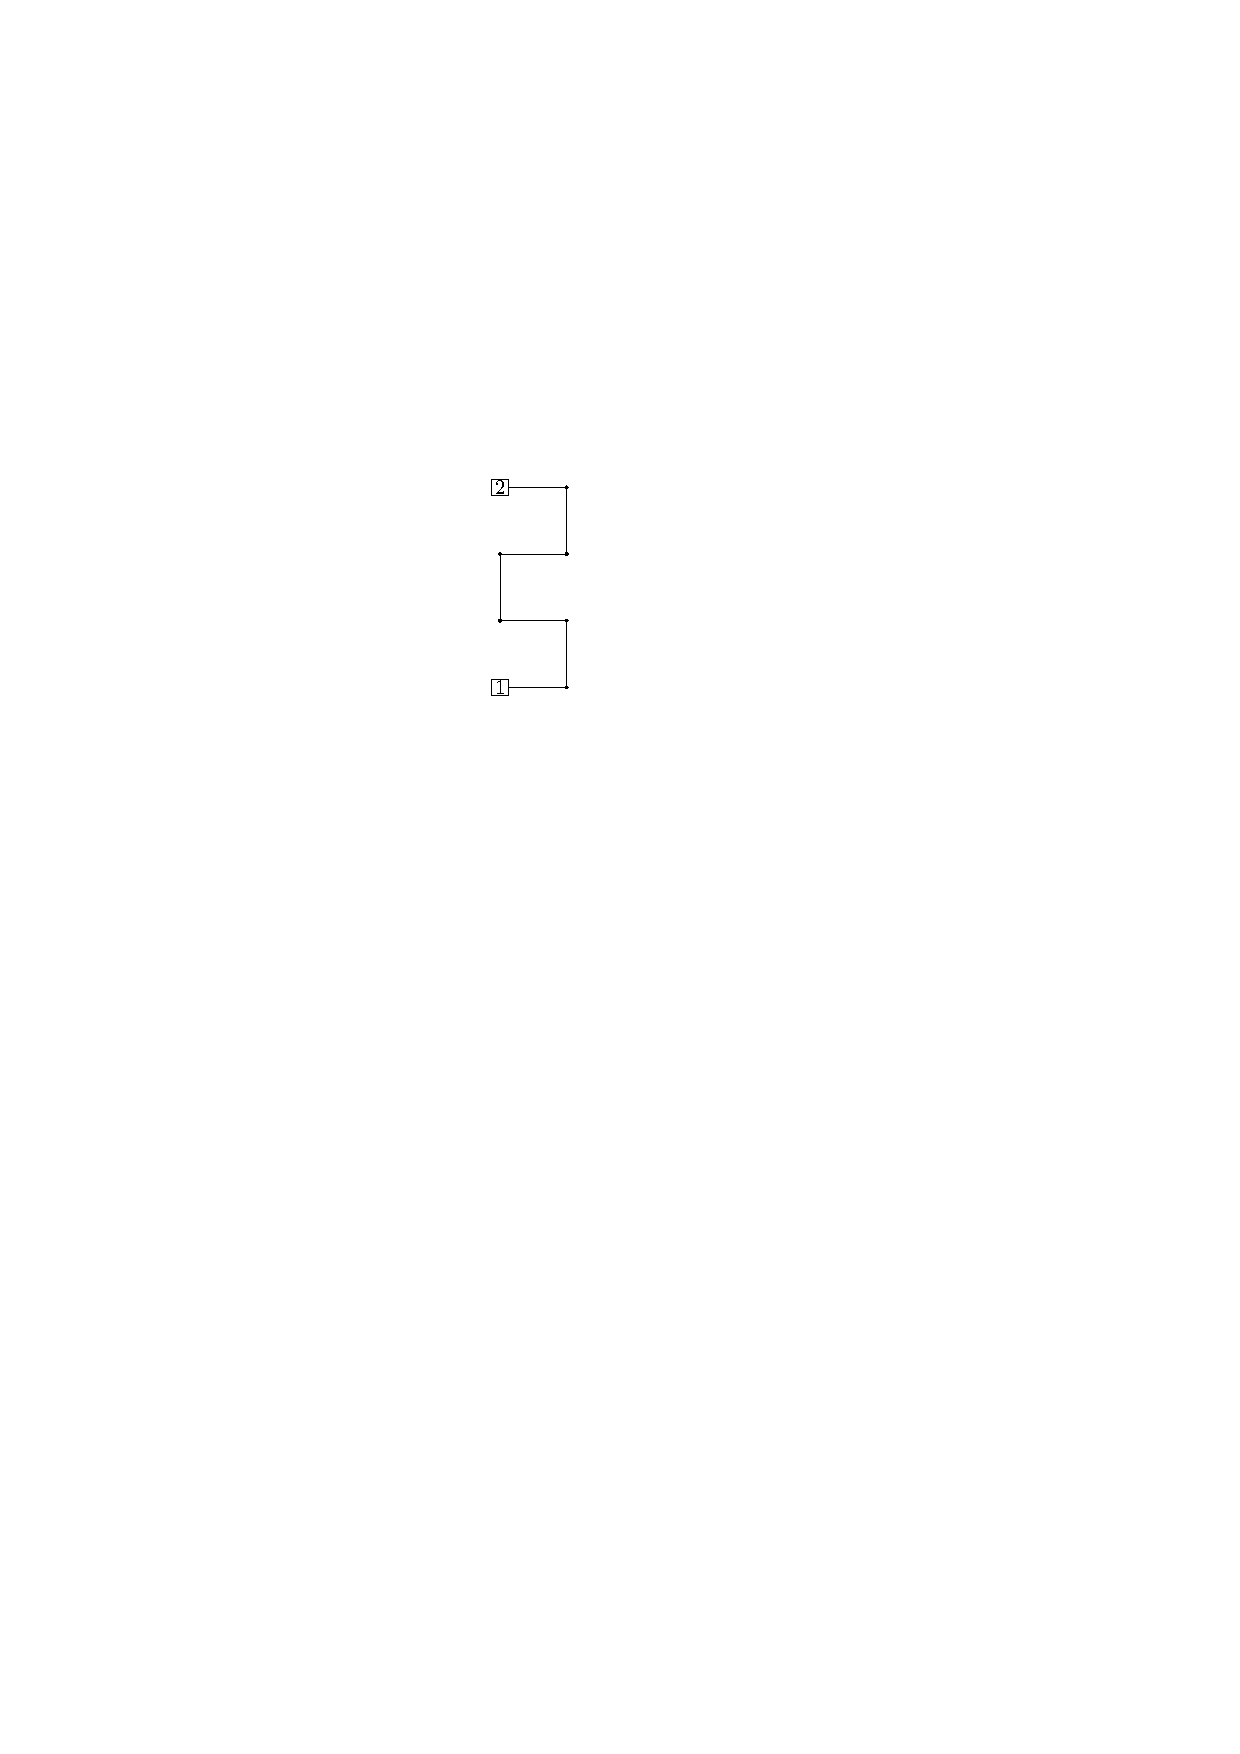
\includegraphics[width=0.4\linewidth,page=1]{includegraphics/bad_2ndfrag.pdf}
		\caption{original input polyedge}\label{im:bad_2ndfrag1}
	\end{subfigure}
	\begin{subfigure}{0.3\textwidth}
		\centering
		\includegraphics[width=0.4\linewidth,page=2]{includegraphics/bad_2ndfrag.pdf}
		
		\caption{Result of algorithm \ref{algo:2ndfrag}}\label{im:bad_2ndfrag2}
	\end{subfigure}
	\begin{subfigure}{0.3\textwidth}
		\centering
		\includegraphics[width=0.4\linewidth,page=3]{includegraphics/bad_2ndfrag.pdf}
		\caption{more appreciating result}\label{im:bad_2ndfrag3}
	\end{subfigure}
	\caption{Bad example of a polyedge for the second uniform-only approach (red highlights the problematic fragment)}
	\label{im:bad_2ndfrag}
\end{figure}
In Figure \ref{im:bad_2ndfrag} the output of Algorithm \ref{algo:2ndfrag} returns uniform-only fragments. The colour highlighting is used this time to illustrate the problem description. In Figure \ref{im:bad_2ndfrag2}, we see that the length of the fragments equals $(3,2,2)$, whereas in Figure \ref{im:bad_2ndfrag3} the individual length is $(3,1,3)$. We are still almost there, although there are situations, where the \grqq bad\grqq~part of a fragmentation is of length one. Still, algorithm \ref{algo:2ndfrag} functions the way we want to. We only have to \textit{recheck} the fragmentation (Line \ref{algo:2ndfrag_recheck} in algorithm \ref{algo:2ndfrag}), whether a fragment of length two can be further minimized by merging the last segment with the next fragment.\\
\begin{algorithm}[H]
	\KwIn{A fragmentation $f$}
	\KwOut{A fragmentation $f$ rechecked}
	\caption{\texttt{recheck}$(f) \in \Rho(k)$\label{algo:recheck}}
	\For{$i = 1$ to $f$\texttt{.length}$-1$}{
		\If{$f_i$.\texttt{length} $= 2$}{
			$v \gets$ first segment of $f_i$\\
			$u \gets$ second segment of $f_i$\\
			\If{$(u)\texttt{.append}(f_{i+1})$\texttt{.uniform} = \texttt{true}}{
				$f_i \gets (v)$\\
				$f_{i+1} \gets (u).\texttt{append}(f_{i+1})$
			}
		}			
	}
	\Return $f$
\end{algorithm}
Obviously, this algorithms runtime is linear to the edge complexity of the input orthogonal polyedge.
\begin{theorem}
	Algorithm \ref{algo:2ndfrag} is sufficient to determine the edge complexity of any polyedge in the smooth orthogonal drawing. Furthermore, the resulting fragmentation can be used to describe a polyedge adequately.
	\label{th:2ndfrag}
\end{theorem}
\begin{proof}
	We already know that uniform fragments do not increase in their complexity and the transition between two incompatible fragments increases the complexity by 1. This leads to a new computation regarding the edge complexity of any polyedge in the smoothened drawing:
	\begin{align}
	ec(f) = \sum_{i = 1}^{f.\texttt{length}} ec(e'_i) + \underbrace{(f.\texttt{length} - 1)}_{\text{fragment transitions}}\label{eq:2ndfrag}
	\end{align}
	The information of alternating fragments does not get lost. By substituting consecutive fragments of up to length two with one big alternating fragment, we are able to describe the behaviour of the polyedge adequately.
\end{proof}
Now we want to establish an algorithm which modifies the fragmentation resulted from algorithm \ref{algo:2ndfrag} to describe the minimum.\\
\begin{algorithm}[H]
	\KwIn{Fragmentation $f$ computed by algorithm \ref{algo:2ndfrag} and \ref{algo:recheck}}
	\KwOut{Minimal fragmentation $e_{\min}$ regarding the relation {\ref{def:ord_rel}}}
	\caption{Min computing of all the fragmentations regarding relation {\ref{def:ord_rel}} \label{al:min_computing}}
	
	$e_{\min} \gets \emptyset$\\
	$f_{\text{alt}} \gets \emptyset$\\
	$f_{\text{alt}}\texttt{.uniform} = \texttt{false}$\\
	\For{$i = 1$ to $f\texttt{.length}$}{
		\If{$f_i\texttt{.length} \geq 3$}{
			\If{$f_\text{alt} \neq \emptyset$}{
				$e_{\min}\texttt{.append}(f_\text{alt})$\\
				$f_\text{alt} \gets \emptyset$
			}
			$f_i\texttt{.uniform} = \texttt{true}$\\
			$e_{\min}\texttt{.append}(f_i)$		
		}
		\Else{
			$f_\text{alt}\texttt{.append}(f_i)$
		}
	}
	\If{$f_\text{alt} \neq \emptyset$}{
		$e_{\min}\texttt{.append}(f_\text{alt})$\\
		$f_\text{alt} \gets \emptyset$
	}
	\Return $e_{\min}$
\end{algorithm}
\subsubsection*{Correctness of algorithm \ref{al:min_computing}}
This algorithm gets the uniform-only fragmentation from algorithm \ref{algo:2ndfrag} as input and determines whether a fragment is of length greater than two. If so, then this fragment is purely uniform and can be considered that way. However, if a fragment is of length one or two, these segments did not fit in any other uniform fragment due to collision reasons. They can be considered as alternating. By using Lemma \ref{lem:alt_2uni}, we know that consecutive fragments of length at most two are analogous to an alternating fragment. This algorithm merges those consecutive segments initialized in line 2-3 and appends them, if a consecutive fragment is of length at least three or there are no further fragments left at the end of the \texttt{for} loop. The longest possible fragmentation given by algorithm \ref{algo:2ndfrag} is of length $\left\lceil\frac{k}{2}\right\rceil$, where $k$ is the complexity of the original orthogonal polyedge and therefore this algorithm also terminates in $\Rho(k)$ runtime.
\begin{theorem}
	The fragmentation resulting from Algorithm \ref{algo:2ndfrag} and \ref{al:min_computing} describes a minimal fragmentation regarding the \textit{FragOrder} relation\label{th:frag_min}
\end{theorem}
\begin{proof}[Proof by contradiction]
	Let $e_{\min}$ be the result of Algorithms \ref{algo:2ndfrag} and \ref{al:min_computing} and $f_{\min}$ be the another valid fragmentation regarding the \textit{FragOrder} relation. Assume that $f_{\min} < e_{\min}$. This would mean that the number of total fragments in $f_{min}$ would be less and the number of alternating fragments are at most the same. This would mean there would be a fragment which can be split into the at most two consecutive fragments. Since Algorithm \ref{algo:2ndfrag} merges uniform ones as long as possible and Algorithm \ref{al:min_computing} merges alternating ones as long as possible, there is no possibility that this fragment could not have been saved beforehand. The same argument holds for the case that $f_{\min}$ would have less alternating fragments. So $f_{\min} \nless e_{\min}$.
\end{proof}
The only thing left to consider is the uniqueness of the computed minimum. We will see that the fragmentations can differ if we change the direction of fragmentation.
\begin{lemma}
	Let $e = (1,2)$ be a polyedge. Then, the optimal fragmentation started at vertex 1 may differ from the fragmentation started at vertex 2.
\end{lemma}
\begin{proof}
	Consider the following example.
	\begin{figure}[H]
		\centering
		\begin{subfigure}{0.3\textwidth}
			\centering
			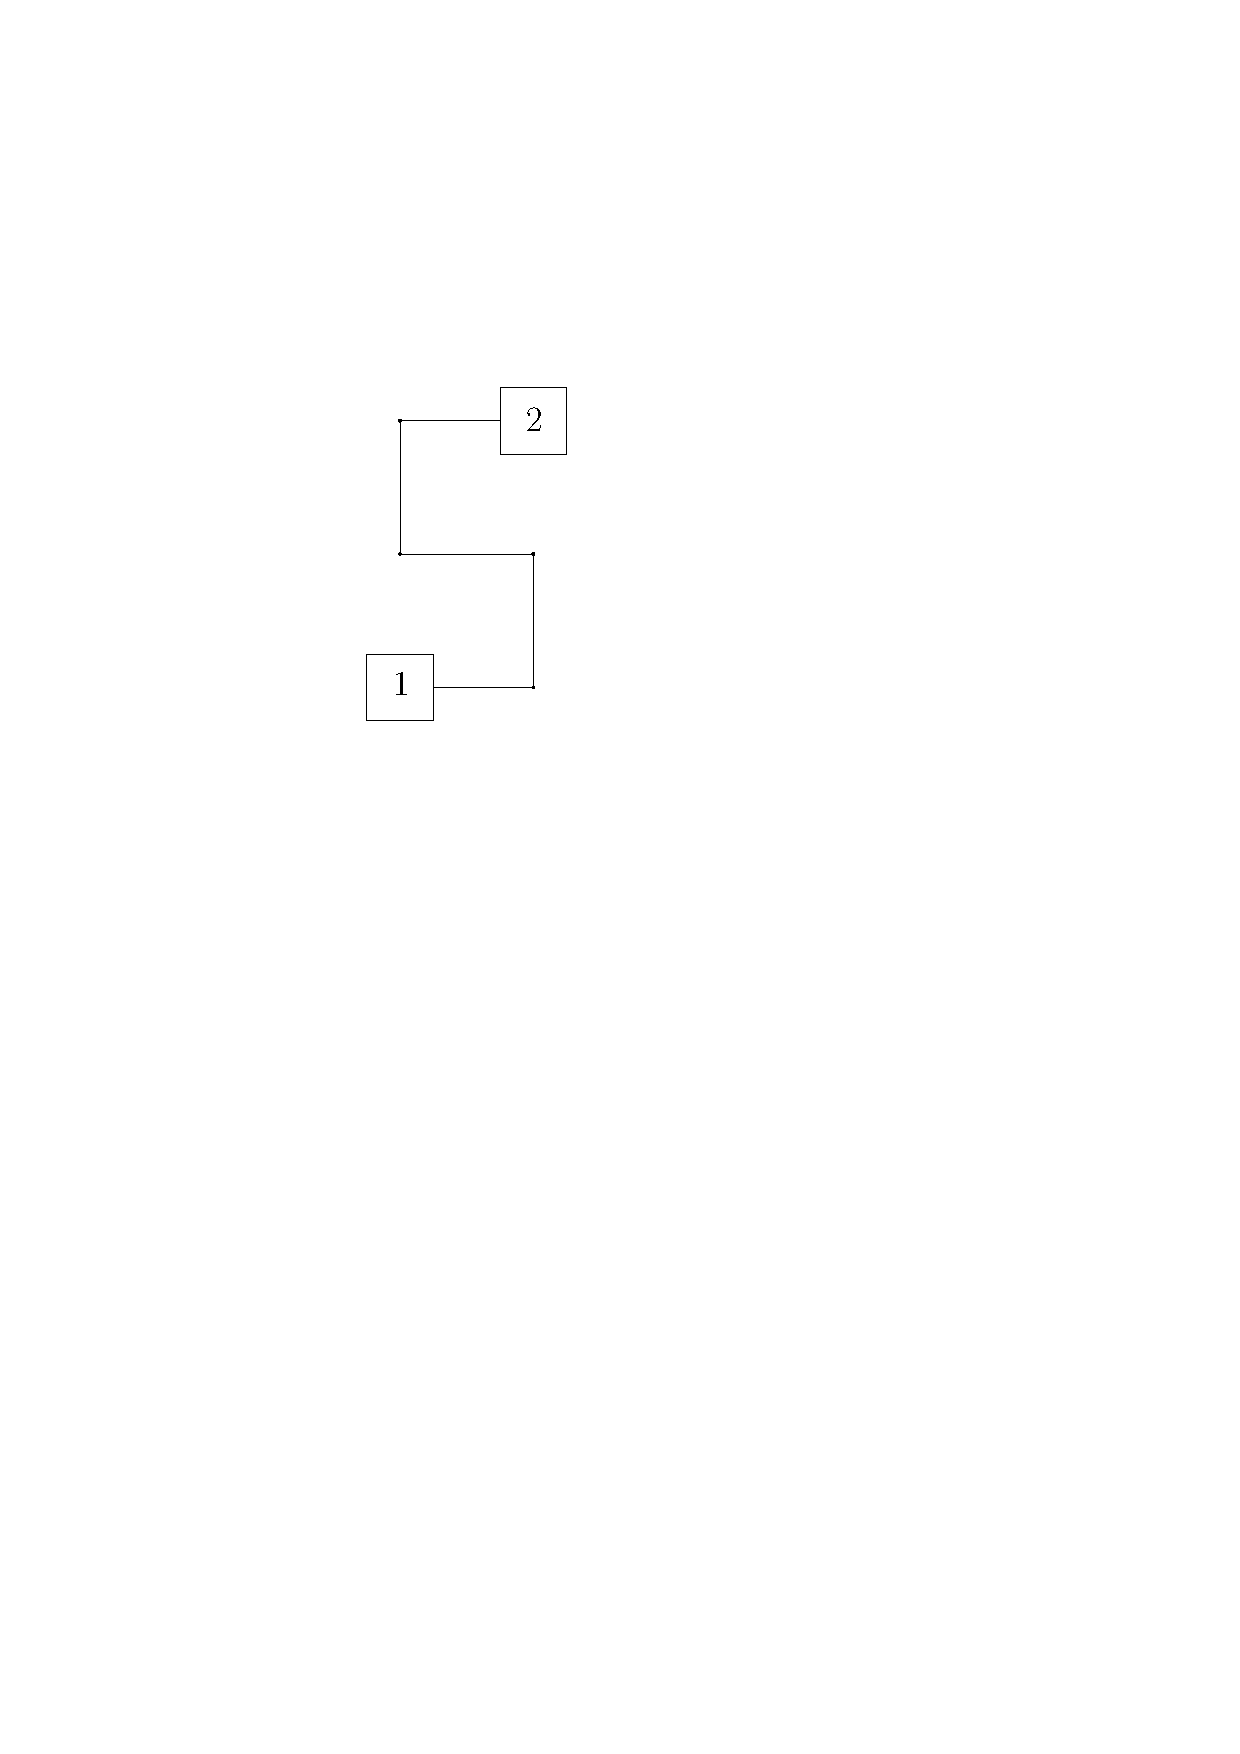
\includegraphics[width=0.4\linewidth,page=1]{includegraphics/non-unique-min.pdf}
			\caption{Input polyedge $(1,2)$}\label{im:non-unique-min1}
		\end{subfigure}
		\begin{subfigure}{0.3\textwidth}
			\centering
			\includegraphics[width=0.4\linewidth,page=2]{includegraphics/non-unique-min.pdf}
			\caption{Fragmented from 1 to 2}\label{im:non-unique-min2}
		\end{subfigure}
		\begin{subfigure}{0.3\textwidth}
			\centering
			\includegraphics[width=0.4\linewidth,page=3]{includegraphics/non-unique-min.pdf}
			\caption{Fragmented from 2 to 1}\label{im:non-unique-min3}
		\end{subfigure}
	\caption{Non-unique optimal fragmentation regarding direction}\label{im:non-unique-min}
	\end{figure}
The fragmentation illustrated in Figure \ref{im:non-unique-min2} from 1 to 2 starts with an uniform fragment of length three, which is not contained in the fragmentation the other way around (Figure \ref{im:non-unique-min3}).
\end{proof}
We see, that the fragmentation is still pretty similar. The next lemma holds the uniqueness of the minimal fragmentation in sense of direction and that the choice of direction does not matter for the validity.
\begin{lemma}
	The fragmentation resulting from algorithm \ref{algo:2ndfrag} and \ref{al:min_computing} is the unique minimum with respect to the direction of the fragmentation. The two minima regarding both fragmentation directions share the same property regarding the number of (alternating) fragments.
\end{lemma}
\begin{proof}
	Consider two fragmentations $f_1$ and $f_2$ regarding the same polyedge $e$, both computed reciprocally with Algorithm \ref{algo:2ndfrag} and \ref{al:min_computing}. Then, Theorem \ref{th:frag_min} holds and the number of alternating fragments and the total number of fragments are of the same size. However, as we saw in Figure \ref{im:non-unique-min}, the fragmentation itself can differ. 
\end{proof}
Now we achieved the best mathematical description of a polyedge in form of a fragmentation. This goes along pretty well with the already achieved results. The results of purely uniform or purely alternating polyedges also apply for purely uniform or purely alternating fragments because every fragment can be considered as a seperate polyedge simulated with dummy vertices. We will see that a fragment with edge complexity $k'$ can be transferred to a SMOG fragment with edge complexity at most $\left\lfloor\frac{3}{2}k'\right\rfloor$. In fact, we will also see that every fragmentation with complexity $k$ will result in a SMOG polyedge with complexity at most $\left\lfloor\frac{3}{2}k\right\rfloor$.
\subsection{Results}
In order to talk about the edge complexity of SMOGs drawings with arbitrary degree we have to consider the number of bends of the polyedges in SMOG. In this section we will look at the possible length of fragmentations, the merge of two fragmentations resulting in one extra bend and will summarize the results.
%\begin{lemma}
%Let $e$ be a polyedge and $e'$ its best fragmentation regarding the number of alternating fragments and total fragments. To be more precise: $e' = \min_{\leq}[e]_{\thicksim_R}$. If the polyedge $e$ does not have a minimal number of bends, $e'$ contains more than one fragment.
%\end{lemma}
\begin{lemma}
	Let $e$ be a polyedge with edge complexity $k$. Then the range of fragmentation lengths is bounded by $\left\lceil\frac{k}{2}\right\rceil$. To be more precise: $$ |e'| \in \left\{1,..., \left\lceil\frac{k}{2}\right\rceil\right\}~~~\forall e'\in [e]_{\thicksim_R} $$
\end{lemma}
\begin{proof}
	If a polyedge with complexity $k$ is purely alternating, then algorithm \ref{algo:frag} will return a valid fragmentation consisting of a single alternating fragment whereas algorithm \ref{algo:2ndfrag} will return a valid fragmentation of $\left\lceil\frac{k}{2}\right\rceil$ fragments. It is possible, that this last fragment is of length one.% or uniform, the minimum fragmentation length of 1 is trivial. Consider the algorithm \ref{algo:frag} given to find a worst case fragmentation. The idea is to create a new fragmentation whenever possible. The first fragment will be of length 3 (initialization of the algorithm), deciding the turn property. The next fragment will get the opposite turn property but will only inherit two segments since the third one will cause a new fragment. The algorithm terminates with either a 2-tuple fragment or a 1-tuple fragment to append. Therefore, there will be at most $\left\lceil\frac{k}{2}\right\rceil$ fragments.
	
	%The $i$-th segment will not fit to the $j$-th fragment considering the turn of $(e_{i-2},e_{i-1},e_i)$. The first fragmentation $e'_1$ consists of three segments. The fourth segment will not fit into the turn property of $e'_1$, a new fragment is created. The fifth segment will fit into $e'_2$ because two segments are violating neither alternating nor uniform turns. The third segment can violate the given turn property though. It is easy to see that the worst case fragmentation starts with a 3-tuple, followed by 2-tuples and ending in either a 2-tuple or a 1-tuple. Therefore, the maximum length of the worst case fragmentation is $\left\lceil\frac{k}{2}\right\rceil$.
\end{proof}
Due to the stretching technique it is guaranteed that every fragment can be substituted with a SMOG fragment.
\begin{lemma}
	The complexity of an orthogonal fragment increases by a factor of $\frac{3}{2}$, iff the fragment is alternating. The complexity does not increase at all, if and only if the fragment is uniform in $\Rho(n^2)\times\Rho(n)$ area.\label{lem:edgebounds}
\end{lemma}
This is a property given by the paper of Bekos et al. and as already proven it does not matter whether the fragments are between other fragments or connected to a vertex. \cite[Figure 6, p. 584]{SMOG}.\\
As seen in Figure \ref{im:incompatible}, the situation arises that one converse bend relative to the others leads to incompatible fragments.
\begin{lemma}
	The transition of two incompatible fragments increases the edge complexity by one bend.\label{lem:transition}
\end{lemma}
\begin{proof}
	If two fragments are incompatible then the degree change between 90\degree~ and 270\degree~result in a circular arc substitution, analoguous to the staircase situation. This results in one more bend per incompatible fragment transition.
\end{proof}
\begin{lemma}
	Let $\Gamma_G$ be a planar orthogonal drawing of a graph $G$ with arbitrary degree. A purely alternating polyedge $e$ with edge complexity $k$ is the worst case situation regarding the number of bends after postprocessing the drawing to a smooth orthogonal drawing. This means that the edge complexity of every polyedge in SMOG is bounded by $\left\lfloor\frac{3}{2}k\right\rfloor$. \label{lem:ec_bound}
\end{lemma}
\begin{proof}
	Consider equation \ref{eq:2ndfrag}, computing the edge complexity of a postprocessed polyedge. At first, let $e$ be a purely alternating polyedge. It follows for its optimal fragmentation:
	\begin{align*}
	\ec(f_e) = \sum_{i=1}^{\left\lceil\frac{k}{2}\right\rceil} \ec(e'_i) + \left\lceil\frac{k}{2}\right\rceil - 1
	\end{align*}
	We have to consider two major cases - $k$ being an even or an odd number.\\
	\underline{$k$ even}\\
	If $k$ is even, then there exists a $n \in \mathbb{N}$ with $k = 2n$. It follows:
	\begin{align*}
	\sum_{i=1}^{n} 2 + n - 1 &= 3n - 1\\
	&= \frac{3}{2}k - 1 < \frac{3}{2}k
	\end{align*}
	\underline{$k$ odd}\\
	If $k$ is odd, then there exists a $n \in \mathbb{N}$ with $k = 2n-1$.
	\begin{align*}
	\sum_{i=1}^{\left\lceil\frac{k}{2}\right\rceil} \ec(f_i) + \left\lceil\frac{k}{2}\right\rceil - 1
	\end{align*}
	If the polyedge is of odd length and purely alternating, then there are $n-1$ fragments of length two and one fragment of length one.
	\begin{align*}
	&\sum_{i=1}^{n-1} 2 + 1 + \left\lceil\frac{k}{2}\right\rceil - 1\\
	= &2n - 2 + 1 + \left\lceil\frac{2n-1}{2}\right\rceil - 1\\
	= &2n - 2 + \left\lceil n-\frac{1}{2}\right\rceil\\
	= &3n-2 = 3\left(\frac{k+1}{2}\right) - 2 = \frac{3}{2}k - \frac{1}{2} = \left\lfloor\frac{3k}{2}\right\rfloor
	\end{align*}
	Now, let $f_e$ be an optimal fragmentation of a non-trivial polyedge $e$ computed by algorithm \ref{algo:2ndfrag}. Then, $e$ is not purely alternating and by Theorem \ref{th:2ndfrag} at least one of the fragments is of length three or greater. 
	\begin{align*}
	\Rightarrow f_e\texttt{.length} < \left\lceil\frac{k}{2}\right\rceil
	\end{align*}
	Longer uniform fragments shall not be a major problem, because their complexity does not increase. On the other hand, by a shorter fragmentation length, we save at least one transition bend mentioned in Lemma \ref{lem:transition}. Now, it immediately follows that the edge complexity does not exceed the staircase situation.
\end{proof}
\begin{theorem}
	Every orthogonal planar drawing of a graph with arbitrary maximum degree can be transferred into a SMOG with the complexity increase bounded by the factor $\frac{3}{2}$ in $\Rho(n^2)\times\Rho(n)$ area.
\end{theorem}
\begin{proof}
	Let $e$ be a polyedge with edge complexity $k$. If $e$ is purely uniform or alternating, Lemma \ref{lem:edgebounds} takes effect and the Theorem is true. If the polyedge is fragmentated non-trivially, we examine the composition with algorithm \ref{algo:2ndfrag} and Lemma \ref{lem:ec_bound} takes effect that the number of bends are bound by the worst case staircase situation. In the previous section, we saw that the area is guaranteed due to the stretching technique and thus planarity is preserved.
	%Thanks to the property of the fragmentation, the worst case would be an initializing fragmentation of the following case: $$\left(\#_{\text{altFrag}}(e') = \#_{\text{uniFrag}}(e')+1\right) \wedge \left(|e'| = \left\lceil\frac{k}{2}\right\rceil\right)$$
	%Examine the edge complexity in SMOG considering the additional bends between all fragments and in alternating fragments. Recall that the edge complexity of $e$ ($\ec(e)$) amounts to $k$ in the Kandinsky model. Consider the worst case fragmentation with  $\left\lceil\frac{k}{4}\right\rceil$ alternating and $\left\lfloor\frac{k}{4}\right\rfloor$ uniform fragments.
	%\begin{align*}
	%k = \sum_{i = 1}^{\left\lceil\frac{k}{4}\right\rceil} \ec(\text{altFrag}_i) + \sum_{j = 1}^{\left\lfloor\frac{k}{4}\right\rfloor} \ec(\text{uniFrag}_j)
	%\end{align*}
	%In SMOG, the complexity increases between two fragments by one bend and in alternating fragments by the factor of $\frac{3}{2}$. Calculate the bound of the \ec(SMOG(e)).
	%\begin{align*}
	%k' &= \frac{3}{2} \cdot \sum_{i = 1}^{\left\lceil\frac{k}{4}\right\rceil} \ec(\text{altFrag}_i) + \sum_{j = 1}^{\left\lfloor\frac{k}{4}\right\rfloor} \ec(\text{uniFrag}_j) + \underbrace{\left\lfloor\frac{k}{2}\right\rfloor-1}_{\text{one bend per transition}}\\
	%&\leq \frac{3}{2} \cdot \sum_{i = 1}^{\left\lceil\frac{k}{4}\right\rceil} \ec(\text{altFrag}_i) + \frac{3}{2} \cdot \sum_{j = 1}^{\left\lfloor\frac{k}{4}\right\rfloor} \ec(\text{uniFrag}_j) = \frac{3}{2} \cdot k
	%	\end{align*}
\end{proof}
These results serve as an upper bound for the worst case of some Kandinsky drawings. In practice, the observations are quite different. Staircase situations only occur up to a certain complexity - for polyedges with higher complexity, it is guaranteed that the shape of the polyedge is mostly uniform. This is due to an optimization in the whole Kandinsky drawing algorithm. The Kandinsky drawings are of course not always computed with a minimal number of bends - as we know, this would be \NP-hard to decide, whether a given graph drawing inhibits the minimal number of bends - but the edge complexity is greedily decreased at a certain point of computation. This leads to a much better upper bound for the edge complexity increase of polyedges.
\begin{lemma}
	Let $k \geq 4$ be the edge complexity of a polyedge $e$ from a Kandinsky drawing $\Gamma_G$ with two Kandinsky bends. Then, the complexity increases to $k+2$ in the smooth orthogonal layout. 
\end{lemma}
\begin{proof}
	$e$ with edge complexity at least 4 has got at most two Kandinsky bends. What lies in between, is purely uniform. Algorithm \ref{algo:2ndfrag} and \ref{al:min_computing} return therefore a fragmentation of length three. At the beginning and the end, there are two alternating fragments of length one, in between lies a purely uniform fragment of length $k-2$. In SMOG, the two Kandinsky bends raise the complexity by one bend. The uniform case does not increase the complexity at all, just as the alternating fragments of length one. Therefore, the edge complexity would increase to $k+2$.
	\begin{align*}
		\left\lfloor\frac{3}{2}k\right\rfloor = k + 2 \Rightarrow k = 4
	\end{align*}
	Therefore, the edge complexity rises by two if the polyedge inhibits at least four segments.
\end{proof}
\section{Saving measures}
\subsection{Introduction}
With our existing approaches we are able to translate any Kandinsky drawing with arbitrary degree to a smooth orthogonal layout with a complexity increase by 2 for larger polyedges in $\Rho(n^2)\times\Rho(n)$ area. The question arises whether it was possible to even save some bends or find a method to stretch with less area requirements in the worst case. In the following section, we examine possibilities to decrease the complexity of polyedges. Furthermore we try to lower the area upper bound in a possible tradeoff with some more bends.
\subsection{Edge Complexity Bounds}
Reconsider the drawing given in Figure \ref{im:kandinsky_bends2}. Due to the fact that the previous results considering 4-planar graphs are also holding for graphs of arbitrary degree, the results are applicable.\\
\begin{figure}[H]
	\centering
	\begin{subfigure}{0.6\linewidth}
		\centering
		\includegraphics[width=0.7\textwidth,page=2]{includegraphics/kandinsky_bends_arbitrary.pdf}
	\end{subfigure}
	\caption{Recall Figure \ref{im:kandinsky_bends2}}\label{im:recall1}
\end{figure}
\begin{theorem}
	Every Kandinsky drawing of a complexity-3 graph with arbitrary degree can be postprocessed to a complexity-4 smooth orthogonal layout in $\Rho(n^2)\times\Rho(n)$ area.
\end{theorem}
\begin{proof}
	Just as the proof of Theorem \ref{th:3to4} holds, the Kandinsky bends are not erasable, leading to a staircase situation of complexity 3. The boxing brings along one more bend, resulting in a polyedge of complexity 4.
\end{proof}
The difference in our new situation is that we are able to reposition the polyedges on the ports. By having a 4-planar graph interpreted in Kandinsky, we are able to connect up to four edges on a single port. This gives us a new opportunity to optimize the drawings.
\begin{remark}
	The \textit{bend or end} property complicates the port reassignment possibilities.
\end{remark}
If we recall Figure \ref{im:kandinsky_bends2}, we could try to alter the port the edge is connected to. Unfortunately, the uniformity of the vertex boxes lead to a possible collision illustrated in Figure \ref{im:bend_or_end_collision}. By doing so, we would further increase the complexity of the edge.
\begin{figure}[H]
	\centering
	\begin{subfigure}{0.3\linewidth}
		\centering
		\includegraphics[width=0.4\textwidth,page=3]{includegraphics/kandinsky_bends_arbitrary.pdf}
		\caption{\textit{bend or end} collision}\label{im:bend_or_end_collision}
	\end{subfigure}
	\begin{subfigure}{0.3\linewidth}
		\centering
		\includegraphics[width=0.4\textwidth,page=4]{includegraphics/kandinsky_bends_arbitrary.pdf}
		\caption{Complexity increase}\label{im:bend_or_end_comp_increase}
	\end{subfigure}
	\caption{Bend or end property complicates matters}\label{im:bend_or_end}
\end{figure}
But on the other hand, the circular arcs are flexible enough to achieve a possible complexity decrease.
\begin{figure}[H]
	\centering
	\begin{subfigure}{0.6\linewidth}
		\centering
		\includegraphics[width=0.7\textwidth,page=5]{includegraphics/kandinsky_bends_arbitrary.pdf}
	\end{subfigure}
	\caption{SMOG complexity decreases}
\end{figure}
However, this is not always possible, as we see in the following Figure:
\begin{figure}[H]
	\centering
	\begin{subfigure}{0.45\linewidth}
		\centering
		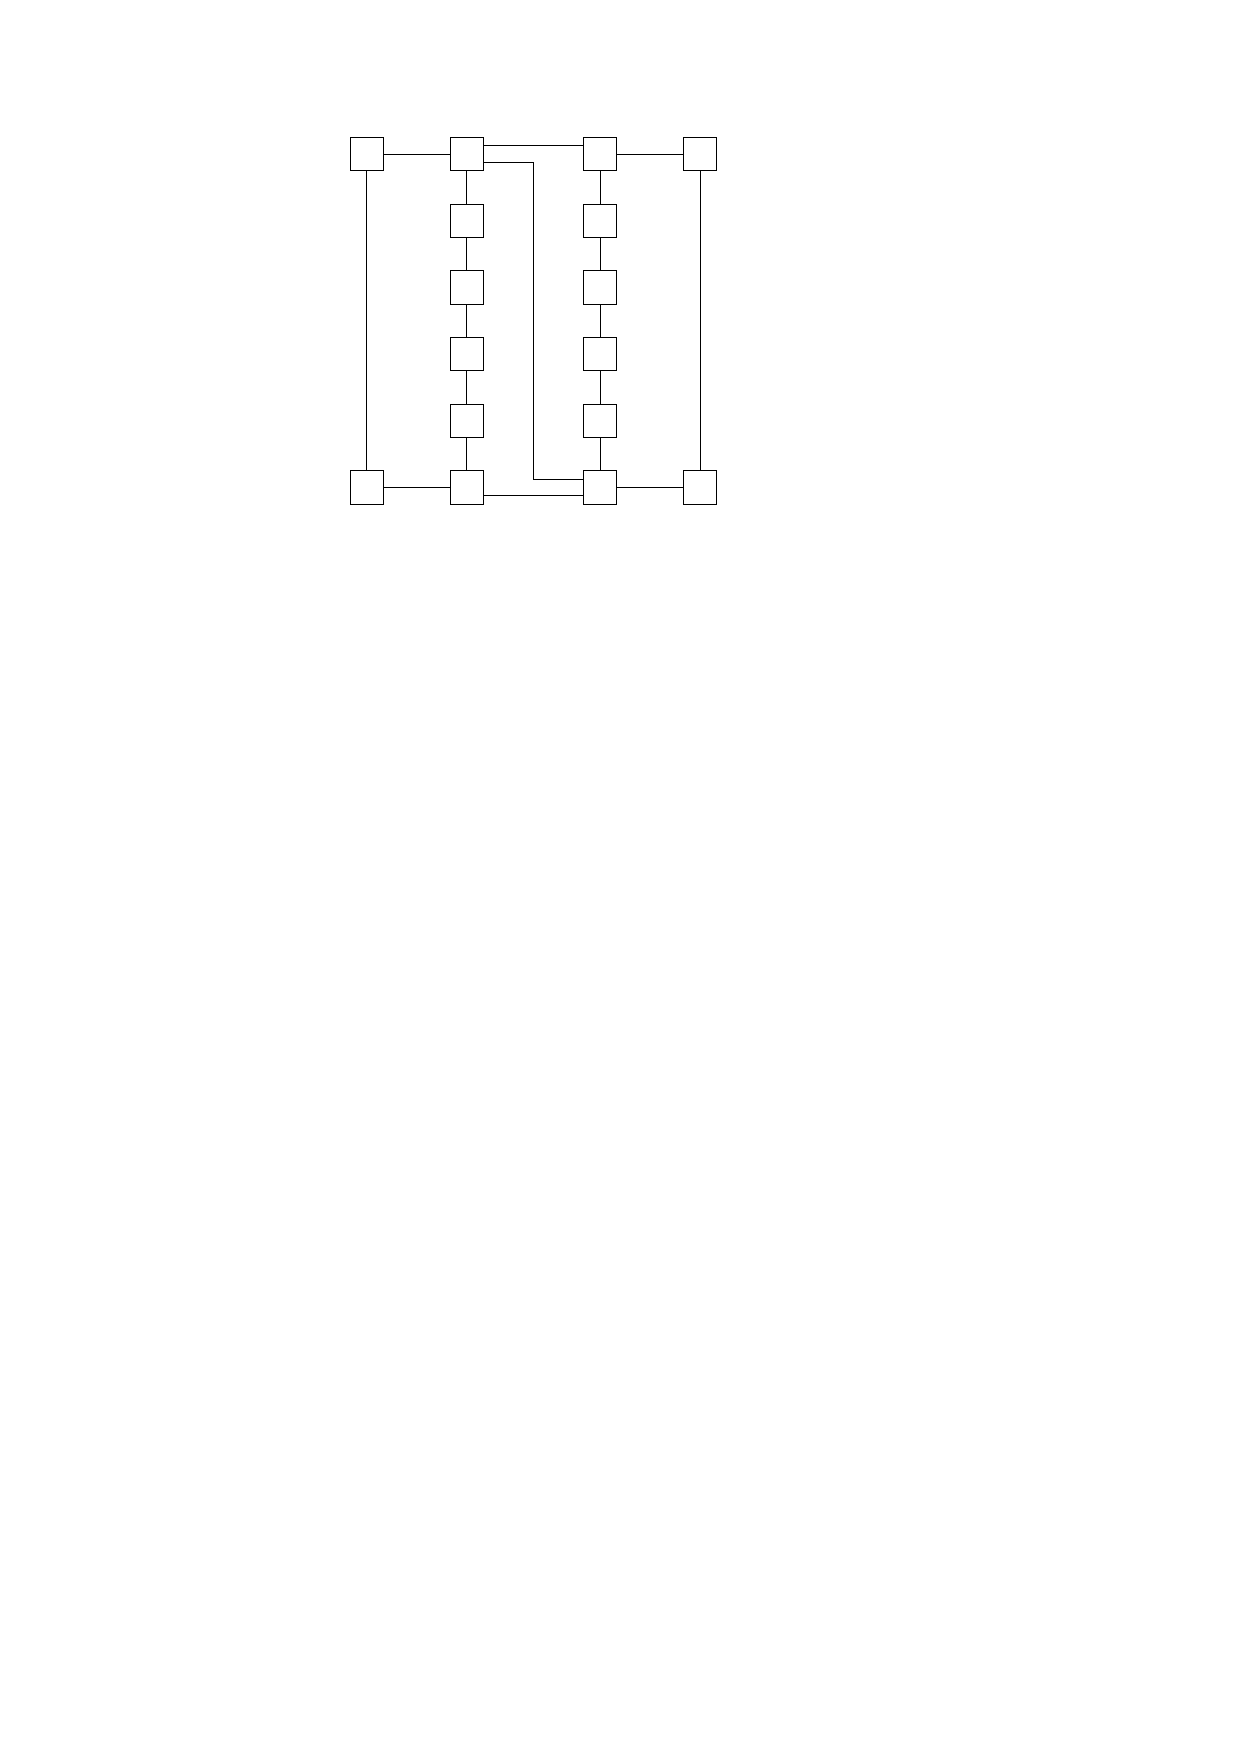
\includegraphics[width=0.45\textwidth,page=1]{includegraphics/port_reassignment_not_possible.pdf}
		\caption{}
	\end{subfigure}
	\begin{subfigure}{0.45\linewidth}
		\centering
		\includegraphics[width=0.7\textwidth,page=2]{includegraphics/port_reassignment_not_possible.pdf}
		\caption{}
	\end{subfigure}
	\caption{This might just be a candidate with negative result}\label{im:port_reassignment_not_possible}
\end{figure}
An approach to find candidate edges for a port reassignment could lie in \grqq half-bends\grqq~and diagonal segments, seen in the $L$ shape and the $T$ shape of the \textit{Kandinsky drawings with almost-empty faces} (Podevsaef drawings in short). In our first approach, we mainly focus on complexity-3 zig zags in the original Kandinsky Model.
\subsubsection{Podevsaef drawings}
Recalling definition \ref{def:podevsaef}, Podevsaef drawings mainly differ from SMOGs in their diagonal segments and 135\degree~bends. The approach to create a Podevsaef drawing is pretty similar to the smooth orthogonal case. At first, the planar Kandinsky drawing of the original graph $G$ is computed which then gets modified by a modification of the \textit{Topology Shape Metrics} algorithm (\cite[p. 4]{podevsaef}). The usage of diagonal segments enable us to illustrate triangular faces with two 135\degree~bends rather than 90\degree~bends. This solution for the bend or end property difficulty enables us to illustrate \textit{almost empty faces}, still inheriting bounding edges with a 0\degree~difference but not orthogonally, therefore \textit{almost} empty. The following solutions were found for $L$ shaped and $T$ shaped triangles:
\begin{figure}[H]
	\centering
	\begin{subfigure}{0.49\linewidth}
		\centering
		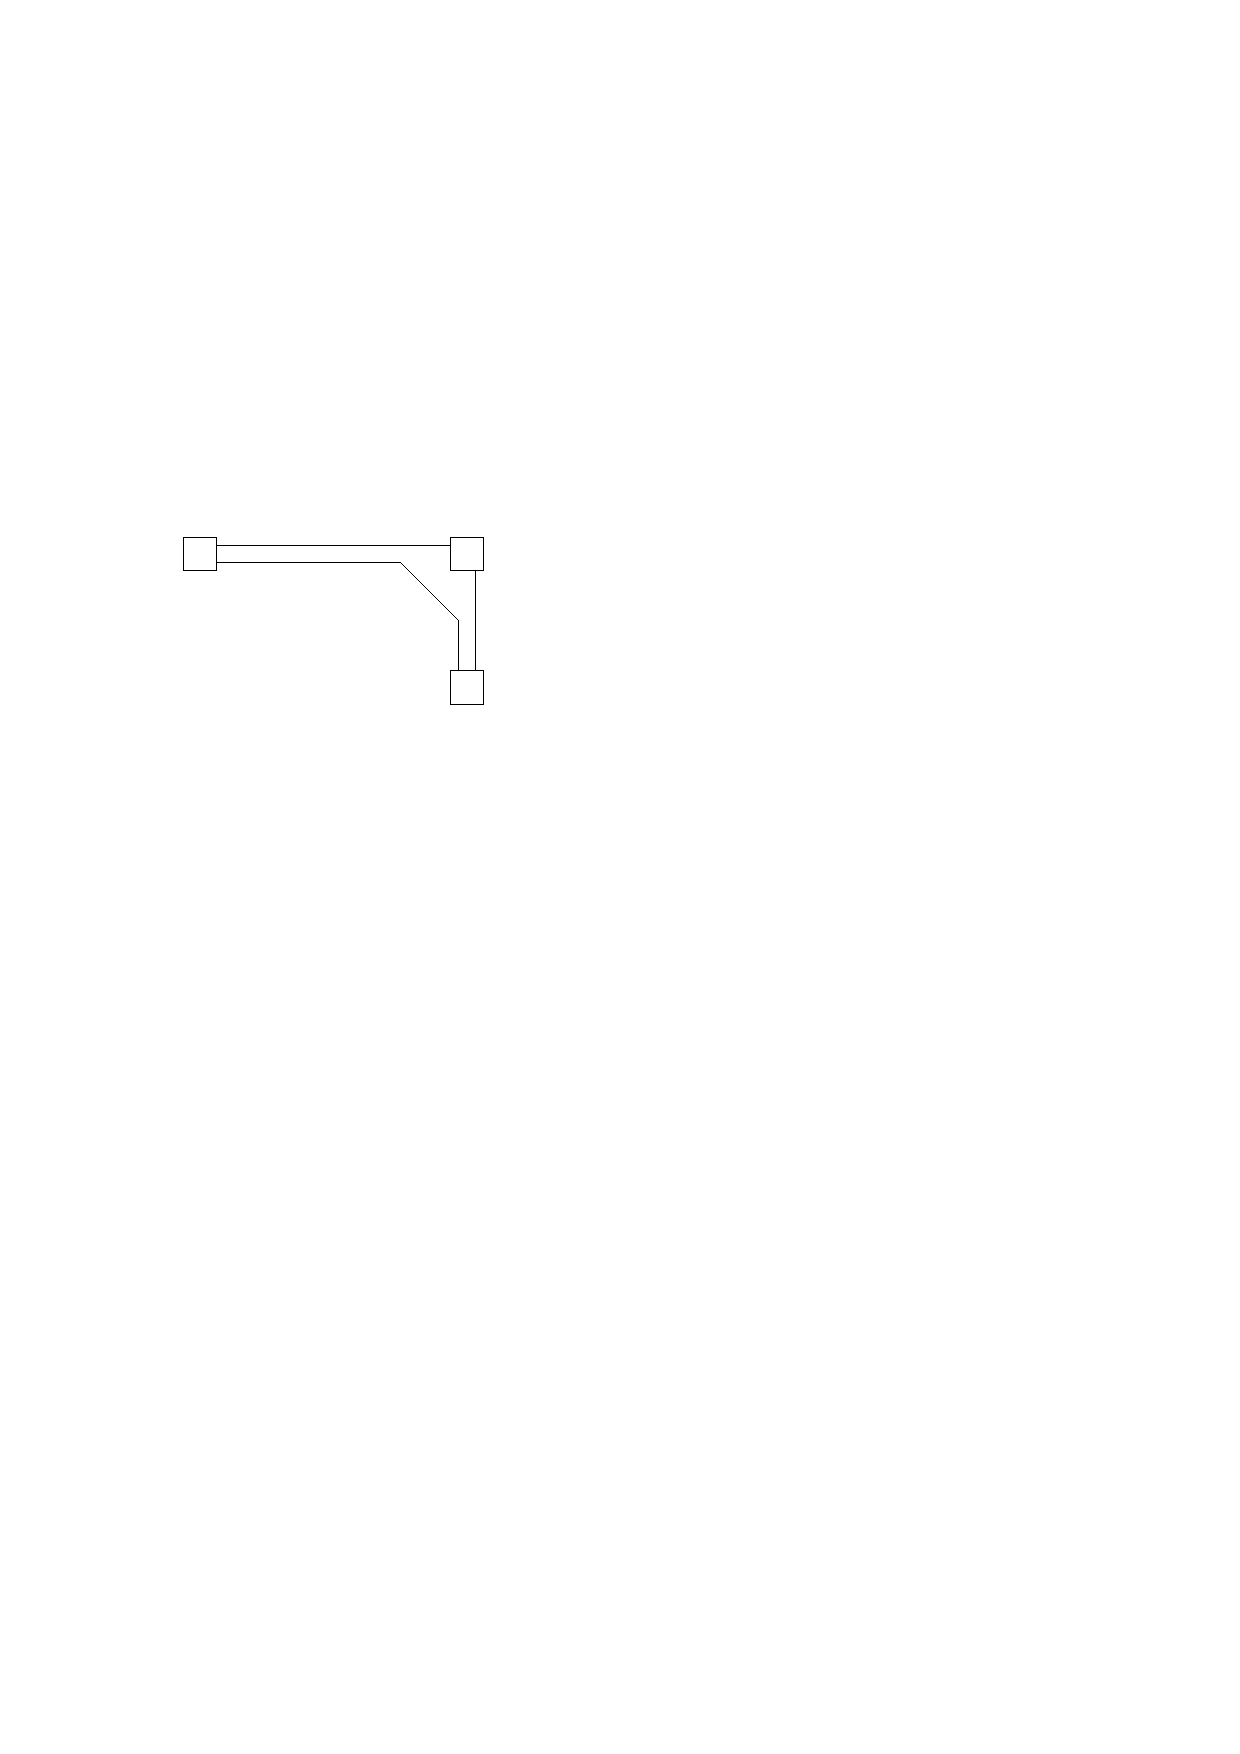
\includegraphics[width=0.471\textwidth,page=1]{includegraphics/L-t-shape_candidates.pdf}
		\caption{}
	\end{subfigure}
	\begin{subfigure}{0.49\linewidth}
		\centering
		\includegraphics[width=0.7\textwidth,page=2]{includegraphics/L-t-shape_candidates.pdf}
	\caption{}
\end{subfigure}
\caption{$L$ and $T$ shapes with almost empty faces}	
\end{figure}
Inspired by this illustration, we look for candidates for possible circular arc substitutions. Both examples from Figure \ref{im:recall1} and Figure \ref{im:port_reassignment_not_possible} might suit for a port reassignment. Although the complexity decrease possibility differs, they both share the achievable planar diagonal half-bend substitution after the application of the stretching technique.
\begin{figure}[H]
	\centering
	\begin{subfigure}{0.2\linewidth}
		\centering
		\includegraphics[width=0.8\textwidth,page=3]{includegraphics/L-t-shape_candidates.pdf}
		\caption{}\label{im:zig-zag_candidates1}
	\end{subfigure}
	\begin{subfigure}{0.39\linewidth}
		\centering
		\includegraphics[width=0.7\textwidth,page=4]{includegraphics/L-t-shape_candidates.pdf}
		\caption{}\label{im:zig-zag_candidates2}
	\end{subfigure}
	\begin{subfigure}{0.39\linewidth}
		\centering
		\includegraphics[width=0.7\textwidth,page=5]{includegraphics/L-t-shape_candidates.pdf}
		\caption{}\label{im:zig-zag_candidates3}
	\end{subfigure}
	\caption{Complexity-3 zig zags examined}\label{im:zig-zag_candidates}	
\end{figure}
\begin{lemma}If a polyedge representation $\Gamma_e$ is zig-zag shaped in Kandinsky (Figure \ref{im:zig-zag_candidates1}) and the port reassignment and circular arc substitution decrease the complexity in the resulting planar SMOG representation (Figure \ref{im:zig-zag_candidates2}), then there is a planar Podevsaef representation with two 135\degree~bends (Figure \ref{im:zig-zag_candidates3}).\label{lem:zig-zag_candidates}
\end{lemma}
So, according to lemma \ref{lem:zig-zag_candidates}, if we look for the possibility of planar Podevsaef polyedge representation like illustrated in figure \ref{im:zig-zag_candidates3} in a polyedge, the port reassignment of one of the vertices might just decrease the complexity. But as we seen, not in every case.
\subsubsection{Using the fragmentation}
Another approach is to use the optimal fragmentation regarding a polyedge to determine whether it was possible to save some bends. The fragmentation itself does not consider the horizontal or vertical alignment of segments in the plane. The following example will motivate the next lemma:
\begin{lemma}
	If the optimal fragmentation of a polyedge contains a fragment of length one in between two other fragments and its line segment is vertical, then the complexity does not increase at this incompatible fragment.
\end{lemma}
\begin{proof}
	Consider the alternating fragment consisting of a single vertical segment in the optimal fragmentation (Figure \ref{im:vertical_fragment2}). Then, the fragments adjacent to it are uniform. Those fragments share the same turn direction because in the uniform-only fragmentation the fragments are alternating their direction of turns. Consider that the original fragment was of length two without the recheck. The next fragment is of length at least three because the fragmentation algorithms have been shifting a second segment. This particular situation enables us to substitute the vertical segment with a half-circular arc due to the same turns of the segments before (Figure \ref{im:vertical_fragment3}). 
\begin{figure}[H]
	\centering
	\begin{subfigure}{0.33\linewidth}
		\centering
		
\includegraphics[width=0.25\textwidth,page=1]{includegraphics/vertical_fragment_1.pdf}
		\caption{}\label{im:vertical_fragment1}
	\end{subfigure}	
	\begin{subfigure}{0.33\linewidth}
		\centering
		
\includegraphics[width=0.25\textwidth,page=2]{includegraphics/vertical_fragment_1.pdf}
		\caption{}\label{im:vertical_fragment2}
	\end{subfigure}
	\begin{subfigure}{0.32\linewidth}
		\centering
		
\includegraphics[width=0.45\textwidth,page=3]{includegraphics/vertical_fragment_1.pdf}
		\caption{}\label{im:vertical_fragment3}
	\end{subfigure}
	\caption{Illustration of the alternating fragment exception}\label{im:vertical_fragment}
\end{figure}
\end{proof}
\subsection{Area Bounds}
In this section, we will examine the possiblities of area bound optimization. Suppose that the original orthogonal drawing is very large and contains a large number of vertices, it is of interest to find a way to lower the upper bound. In the first approach, we will erase redundancies in a drawing with a plane sweep method. In the second approach, we will substitute the circular arcs with ellipses or specific segment combinations in order to lower the upper bound by $\Rho(\sqrt{n})$, which may increase the lower bound of the edge complexity on the other hand.
\subsubsection*{Plane sweep erasing}
The stretching technique does not increase the edge complexity excessively. On the other hand, it may appear that the horizontal area expansion of a drawing is unnecessarily big. In this section, a linear runtime plane sweep may be a stable solution regarding area and even edge complexity retrenchment. Consider the following example:
\begin{figure}[H]
	\centering
	\begin{subfigure}{0.33\linewidth}
		\centering
		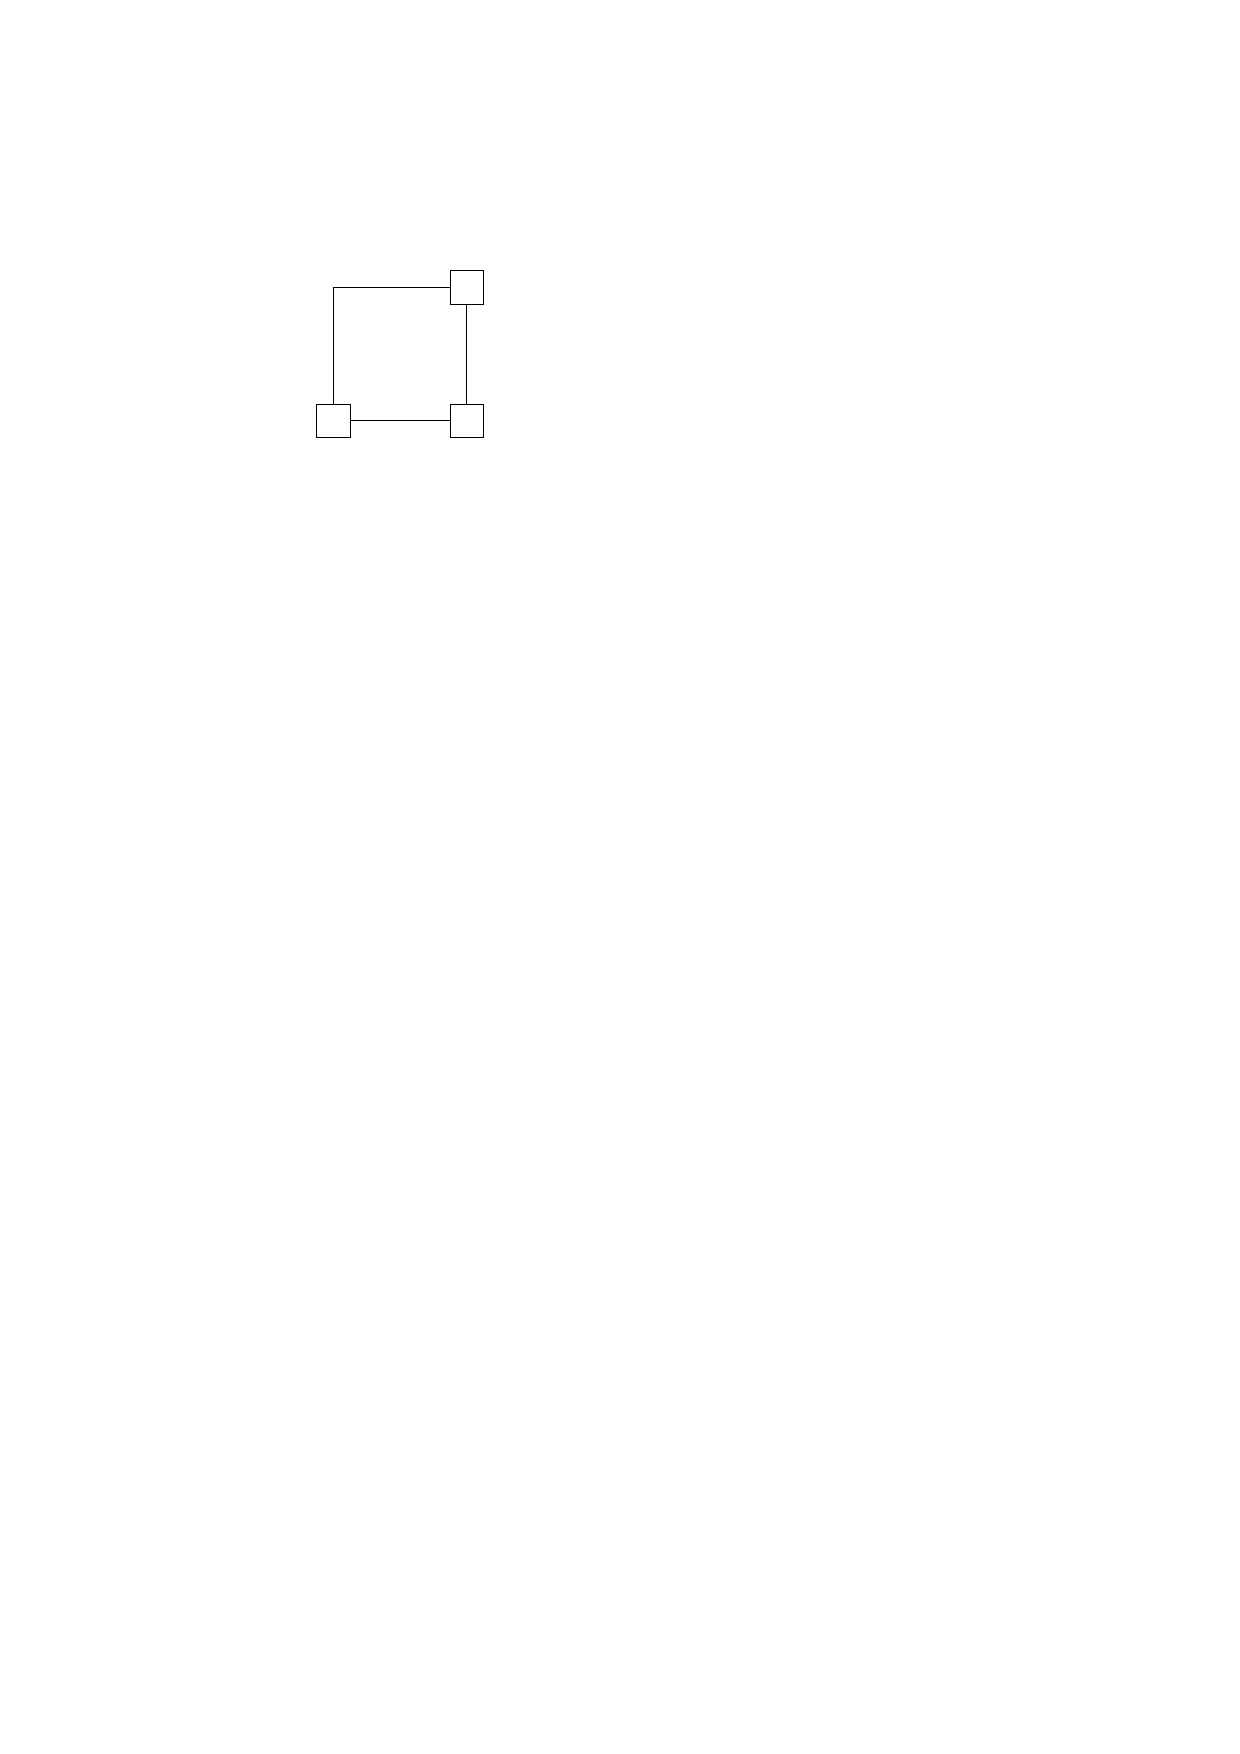
\includegraphics[width=0.4\textwidth,page=1]{includegraphics/plane_sweep_save.pdf}
		\caption{}
	\end{subfigure}	
	\begin{subfigure}{0.33\linewidth}
		\centering
		\includegraphics[width=0.8\textwidth,page=2]{includegraphics/plane_sweep_save.pdf}
		\caption{}
	\end{subfigure}
	\begin{subfigure}{0.32\linewidth}
		\centering
		\includegraphics[width=0.4\textwidth,page=3]{includegraphics/plane_sweep_save.pdf}
		\caption{}
	\end{subfigure}

	\caption{One plane sweep could eradicate redundant area and even segments without causing any damage}\label{im:sweep_save}
\end{figure}
As you can see in Figure \ref{im:sweep_save}, an orthogonal Kandinsky drawing of a triangle gets transferred to a smooth orthogonal drawing in the Fixed Shape Model. The vertical orange-colored lines show the possible saving of area. Even one horizontal segment is eliminated in the process, reducing the complexity of the drawing to one.
\begin{definition}
	There is a plane sweep algorithm which eliminates unnecessary space and may even save some segments in linear runtime regarding the size of the drawing. The vertical segments do not have to be considered by the plane sweep.
\end{definition}
This plane sweep algorithm identifies the presence of \textit{vertices} and \textit{circular arcs} as an event. Obviously, it is undesirable to interfere with circular arcs while cutting the drawing. First we show, that considering vertices, circular arcs and horizontal line segments is sufficient.\\
The \textit{vertical line segments} are not to be considered because either they end in one or two vertices. This means that vertices are sufficient in this case to be seen. If a vertical line segment is not connected to any vertex, then, by definition of the SMOG Model, they are connected to circular arcs which are also considered by the sweep line.\\
The horizontal segments are part of the events in order to determine which segments can be cut between two events. The plane sweep iterates from the left side to the right and is able to delete unnecessary horizontal redundancy with one sweep. Therefore, this plane sweep will run in linear runtime regarding the size of the drawing.
\begin{lemma}
	This area saving plane sweep is able to save up to $\Rho(\sqrt{w})$ area, where $w$ is the width of the input drawing and it potentially lowers the overall complexity of a drawing.
\end{lemma}
\begin{proof}
	Consider following orthogonal drawing of the graph:
	\begin{figure}[H]
		\centering
		\begin{subfigure}{0.45\linewidth}
			\centering
			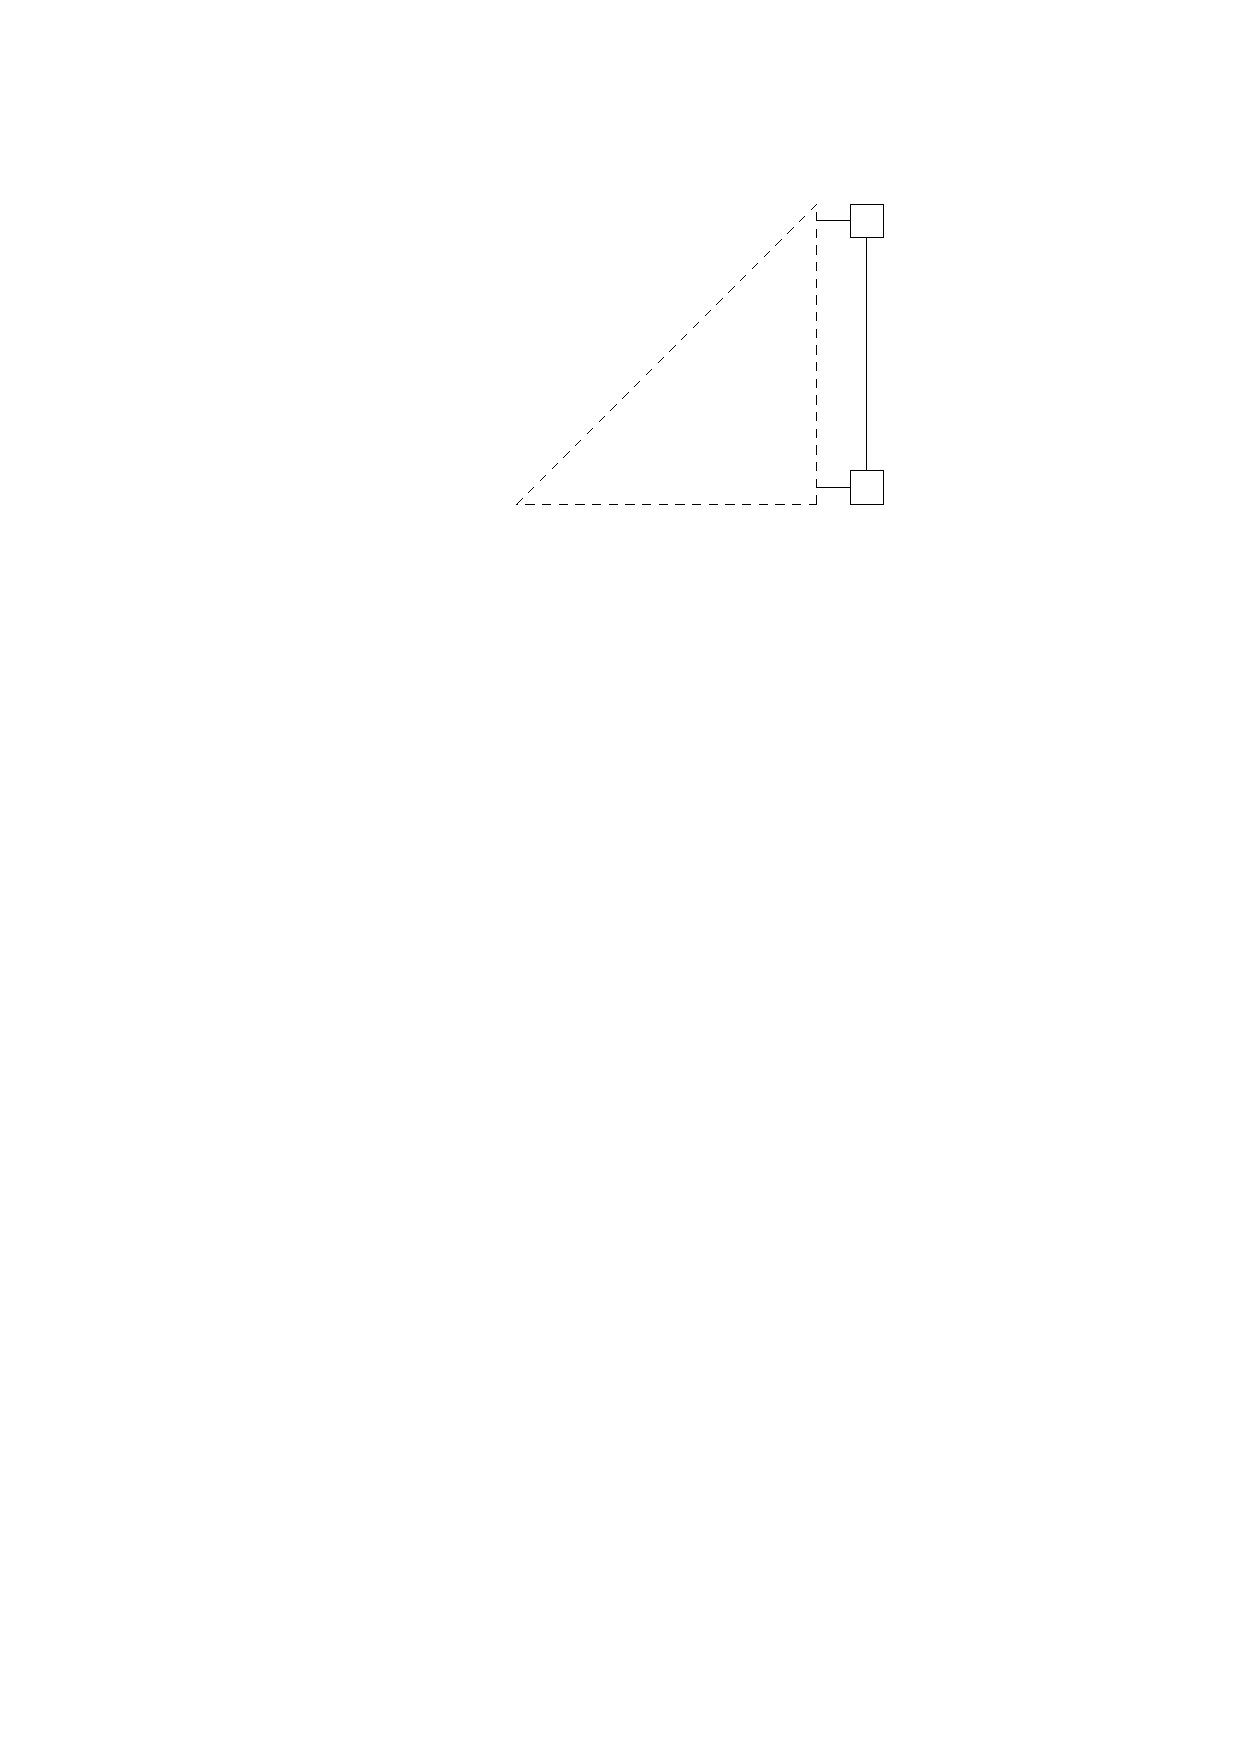
\includegraphics[width=0.5\textwidth,page=1]{includegraphics/plane_sweep_linear_saving.pdf}
			\caption{}\label{im:ortho_max_saving1}
		\end{subfigure}	
		\begin{subfigure}{0.4\linewidth}
			\centering
			\includegraphics[width=0.5\textwidth,page=2]{includegraphics/plane_sweep_linear_saving.pdf}
			\caption{}\label{im:ortho_max_saving2}
		\end{subfigure}
	\caption{Orthogonal drawing with maximal saving possibilites}\label{im:ortho_max_saving}
	\end{figure}
The dotted triangle of figure \ref{im:ortho_max_saving1} consists of $\Rho(n)\times\Rho(n)$ vertices as illustrated in figure \ref{im:ortho_max_saving2}. Applying the stretching technique and circular arc substitution, the resulting SMOG drawing is of size $\Rho(n^2)\times\Rho(n)$.
	\begin{figure}[H]
	\centering
	\begin{subfigure}{0.45\linewidth}
		\centering
		\includegraphics[width=0.7\textwidth,page=3]{includegraphics/plane_sweep_linear_saving.pdf}
		\caption{}\label{im:ortho_max_saving3}
	\end{subfigure}	
	\begin{subfigure}{0.4\linewidth}
		\centering
		\includegraphics[width=0.7\textwidth,page=4]{includegraphics/plane_sweep_linear_saving.pdf}
		\caption{}\label{im:ortho_max_saving4}
	\end{subfigure}
	\caption{SMOG drawing with maximal saving possibilites}
\end{figure}
In figure \ref{im:ortho_max_saving4}, the orange dotted lines indicate where the area saving plane sweep triggers an event. Notice that there are $\Rho(n)$ events.
	\begin{figure}[H]
	\centering
	\begin{subfigure}{0.45\linewidth}
		\centering
		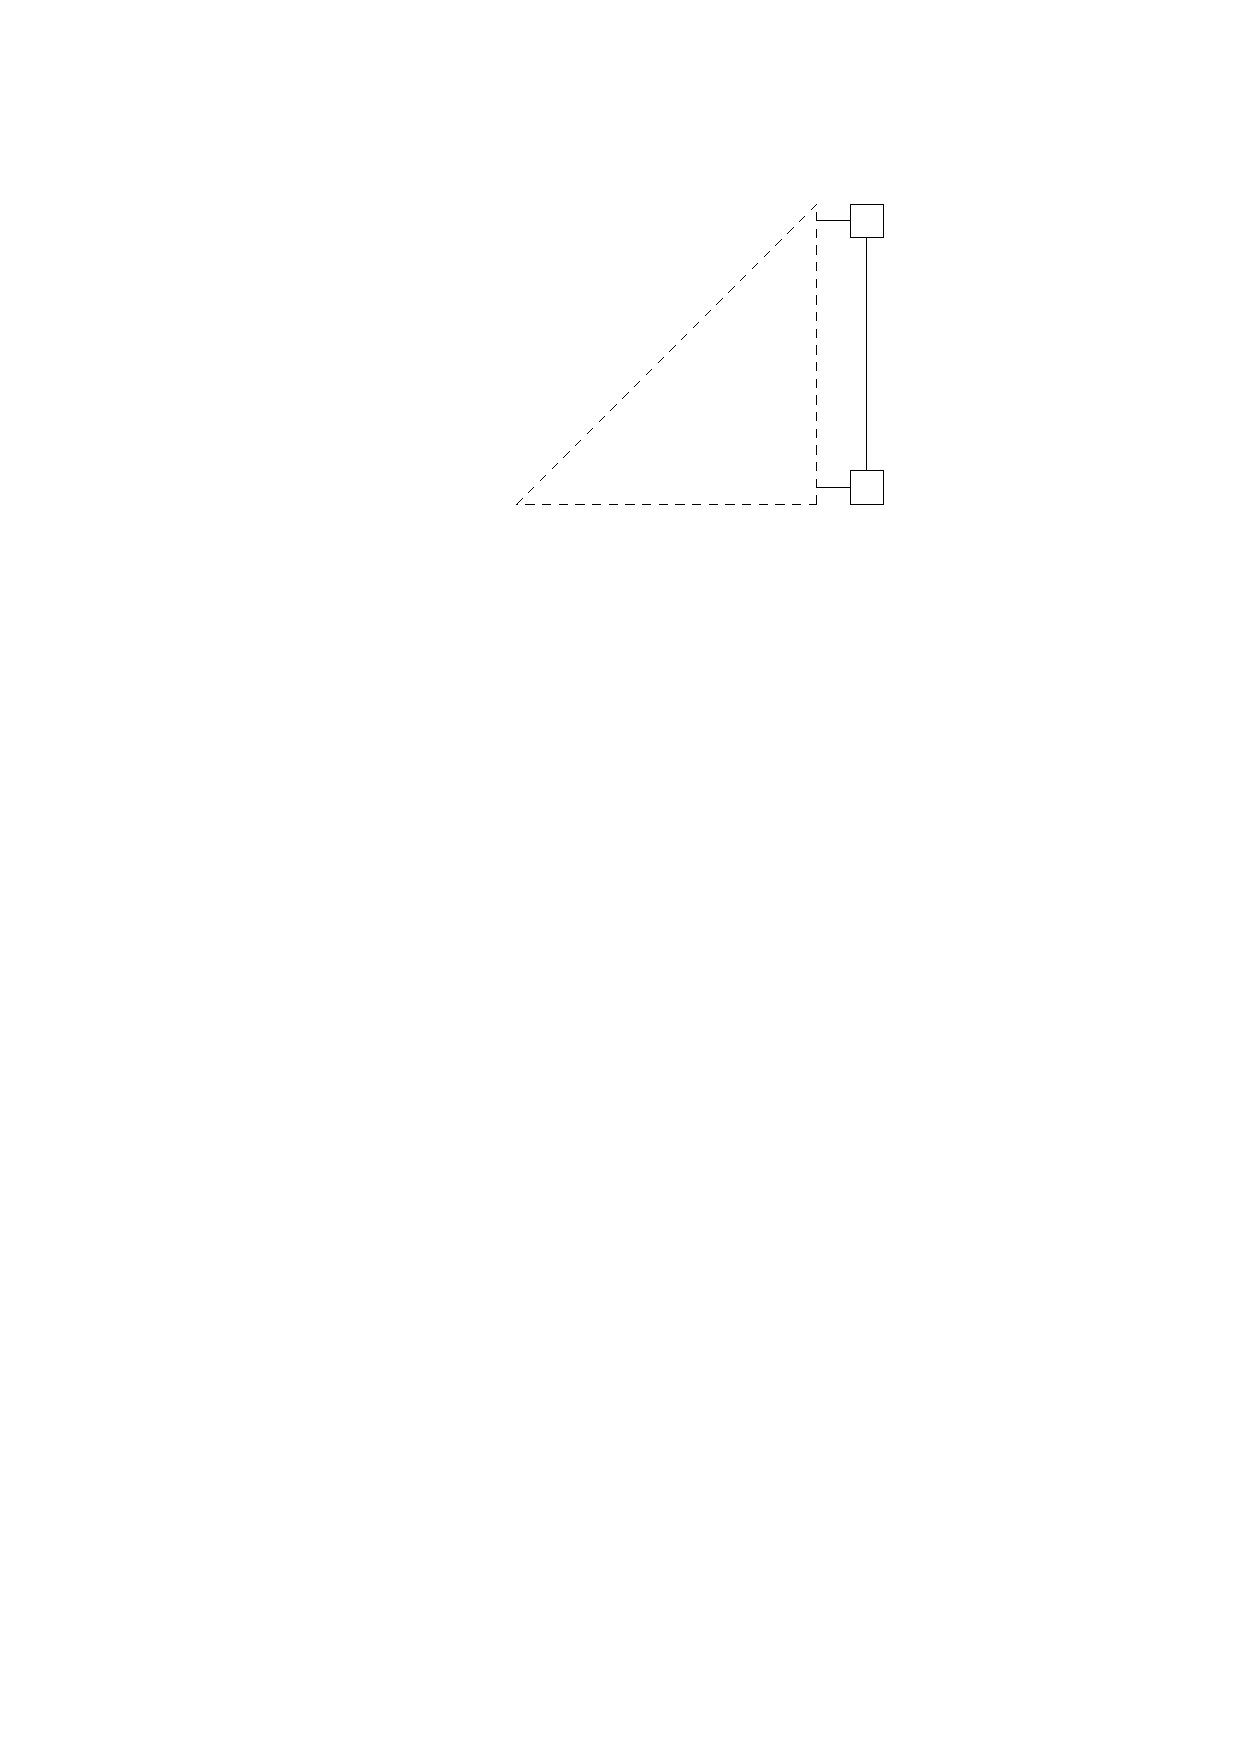
\includegraphics[width=0.5\textwidth,page=1]{includegraphics/plane_sweep_linear_saving.pdf}
		\caption{}
	\end{subfigure}	
	\begin{subfigure}{0.4\linewidth}
		\centering
		\includegraphics[width=0.5\textwidth,page=5]{includegraphics/plane_sweep_linear_saving.pdf}
		\caption{}\label{im:ortho_max_saving5}
	\end{subfigure}
	\caption{SMOG drawing after applying the plane sweep}
\end{figure}
After cutting area redundancies, we decrease the complexity of the graph to one and save $\Rho(n)$ area horizontally.
\end{proof}
However, the plane sweep will not work properly in all scenarios, as the following example will show:
\begin{figure}[H]
	\centering
	\begin{subfigure}{0.5\linewidth}
		\centering
		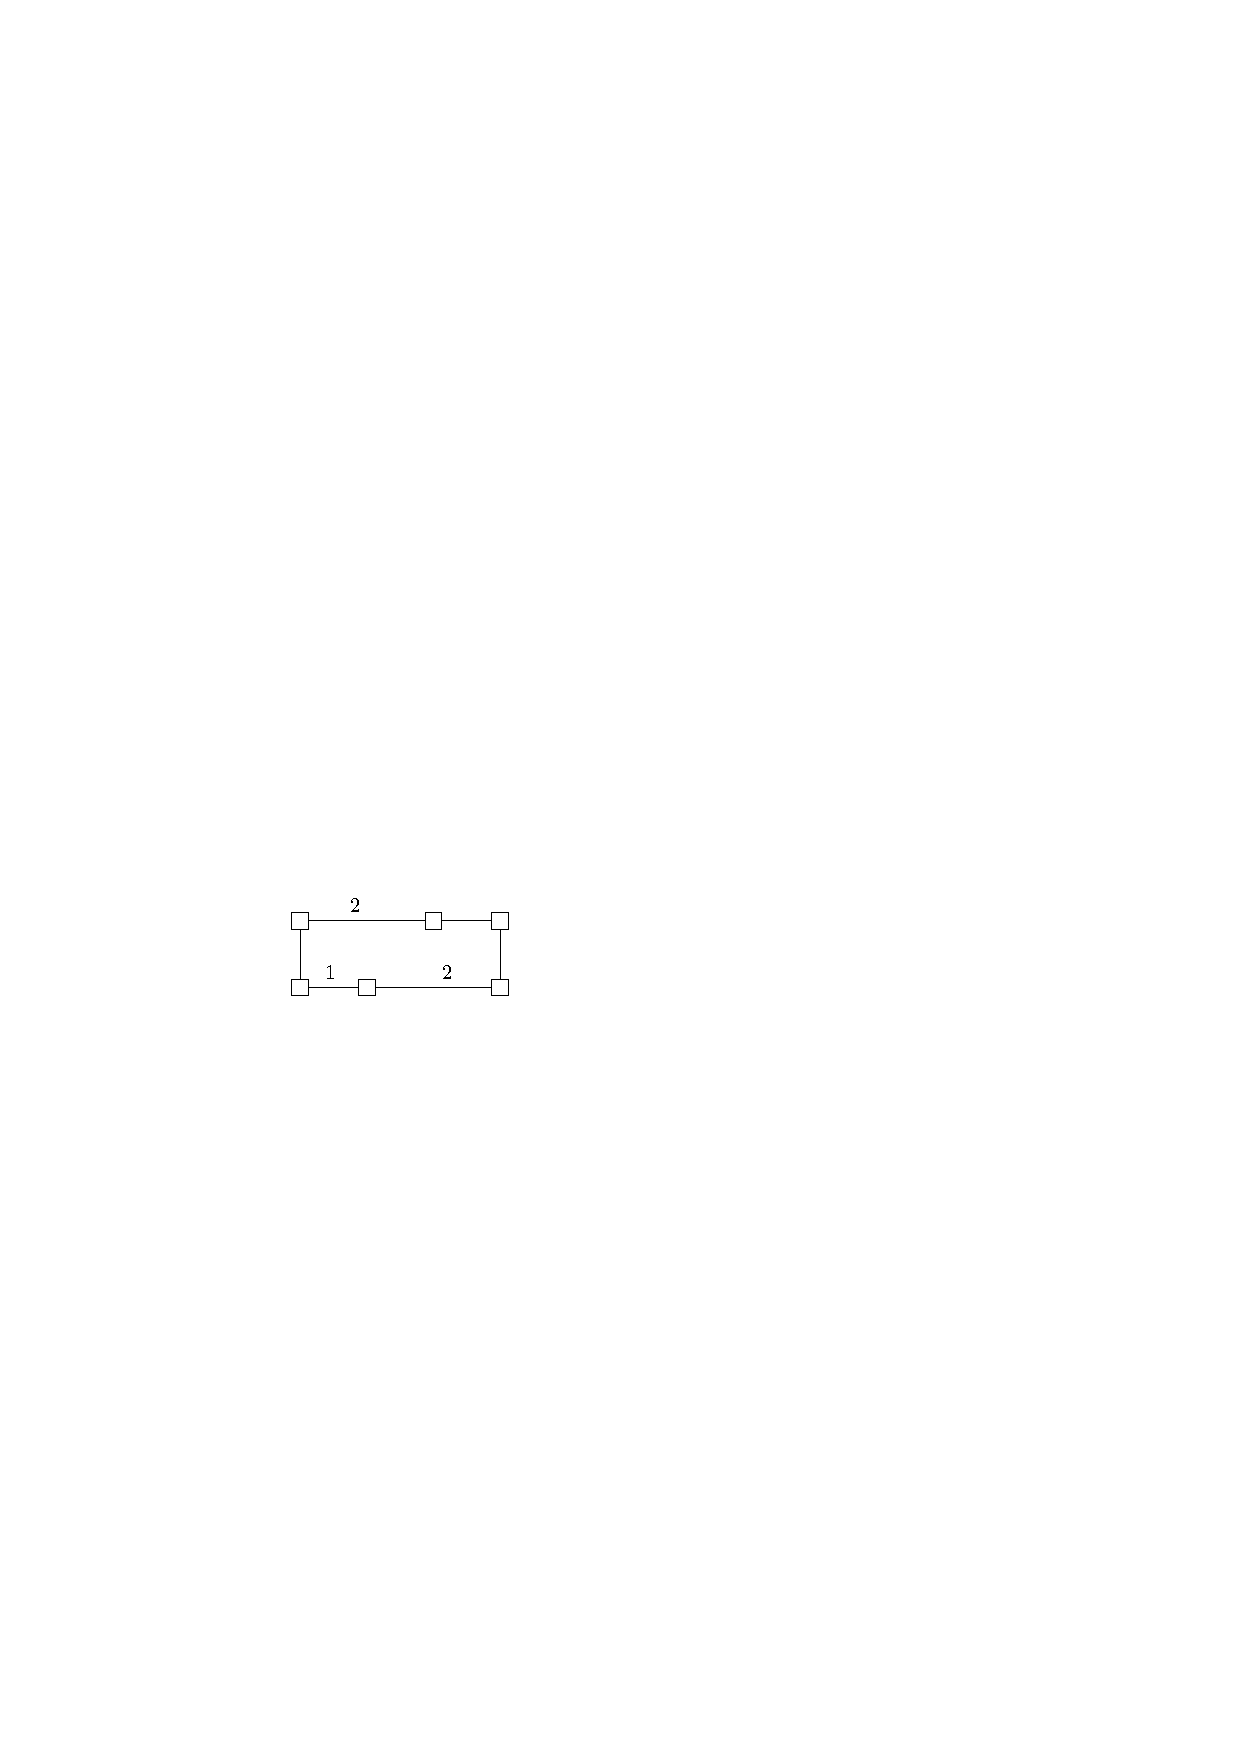
\includegraphics[width=0.6\textwidth,page=1]{includegraphics/plane_sweep_not_working.pdf}
	\end{subfigure}
	\caption{The plane sweep will not reduce anything}\label{im:plane_sweep_bad_example1}
\end{figure}
Consider the drawing in Figure \ref{im:plane_sweep_bad_example1} with a unit length of 1. While iterating from left to right, there will be a vertex as a new event with unit length difference to the last event. However, this drawing can be optimized regarding horizontal area as shown in figure \ref{im:plane_sweep_bad_example2}.
\begin{figure}[H]
	\centering
	\begin{subfigure}{0.5\linewidth}
		\centering
		\includegraphics[width=0.6\textwidth,page=2]{includegraphics/plane_sweep_not_working.pdf}
	\end{subfigure}
	\caption{Optimized drawing derived from figure \ref{im:plane_sweep_bad_example1}}
	\label{im:plane_sweep_bad_example2}
\end{figure}
In order to find a solution for this situation, a new approach based on the \textit{4M} algorithm is formulated.
\subsubsection{Modified 4M - Moving}
Recalling section \ref{section:4M}, the 4M algorithm consists of multiple operations. In this section, we will consider the \textit{moving} operation. 
\subsubsection*{Model consistency}
It is to examine whether the \textit{4M} operations were suitable for drawings which underly the Kandinsky model. In the Kandinsky model, the vertices are represented with boxes of uniform size. In the orthogonal 4M model, the boxes have to overlap the grid lines by $\frac{\lambda}{4}$, and the rectangles were of size $\left(w\lambda-\frac{\lambda}{2} \right)\times \left( h\lambda-\frac{\lambda}{2}\right);w,h\in\mathbb{N}$. By setting $w = h = 1$, we achieve a consistency with the Kandinsky model and therefore can continue examining a 4M algorithm modification.
\subsubsection*{The modification}
The focus lies in the horizontal area saving. The moving line $J$ will still be directed and starts above to topmost object and ends below the bottommost object of the drawing. Considering orthogonal graphs, $J$ only crosses horizontal lines from top to bottom. In the smoothened Kandinsky case, quarter circular arcs traverse in height and width - so they also have to be crossed for total area savings. 
\begin{figure}[H]
	\centering
	\begin{subfigure}{0.4\linewidth}
		\centering
		\includegraphics[width=0.4\textwidth,page=1]{includegraphics/4M_Moving_arcs.pdf}
		\caption{$J$ crossing the drawing}
	\end{subfigure}
	\begin{subfigure}{0.4\linewidth}
		\centering
		\includegraphics[width=0.2\textwidth,page=2]{includegraphics/4M_Moving_arcs.pdf}
		\caption{Circular arc substitution}
	\end{subfigure}
	\caption{A first, easy example}\label{im:arc-crossing_example1}
\end{figure}
As you can see in figure \ref{im:arc-crossing_example1}, a quarter circular arc with radius $r$ can be reduced in width by substituting with a circular arc with radius $r-c\cdot\lambda$ and a vertical segment of length $c\cdot\lambda$. $\lambda$ describes the unit length, $c$ describes the amount of unit reducings possible along $J$. By this method, the complexity may increase by one per crossed quarter circular arc. 
\begin{figure}[H]
	\centering
	\begin{subfigure}{0.4\linewidth}
		\centering
		\includegraphics[width=0.4\textwidth,page=3]{includegraphics/4M_Moving_arcs.pdf}
		\caption{$J'$ crossing the drawing}\label{im:arc-crossing_example2a}
	\end{subfigure}
	\begin{subfigure}{0.4\linewidth}
		\centering
		\includegraphics[width=0.265\textwidth,page=4]{includegraphics/4M_Moving_arcs.pdf}
		\caption{Quarter circular arc substitution}
	\end{subfigure}
	\caption{A second example}\label{im:arc-crossing_example2}
\end{figure}
In this example, $J'$ crosses two consecutive quarter circular arcs in a drawing of size $6\times6$. The result is a drawing of size $4\times6$, with an edge complexity of three. A verticel line segment of length one is introduced per substituted arc, merged to a vertical line segment of length two.\\
To further decrease the area of the drawing, a horizontal path from the leftmost object to the rightmost one would reduce and even eliminate the vertical line segments crossed by $J'$.
\begin{figure}[H]
	\centering
	\begin{subfigure}{0.4\linewidth}
		\centering
		\includegraphics[width=0.7\textwidth,page=5]{includegraphics/4M_Moving_arcs.pdf}
		\caption{$J'$ crossing the drawing}
	\end{subfigure}
	\begin{subfigure}{0.4\linewidth}
		\centering
		\includegraphics[width=0.7\textwidth,page=6]{includegraphics/4M_Moving_arcs.pdf}
		\caption{Circular arc substitution}
	\end{subfigure}
	\caption{Vertical area saving}\label{im:arc-crossing_example3}
\end{figure}
The area bounds of the drawing from Figure \ref{im:arc-crossing_example2a} can further be reduced by a horizontal moving line $J'$, resulting in a $4\times4$ drawing. In order to do so, one has to \textit{reduce the line segment between quarter circular arcs first}. This results in a possible complexity decrease, in this case a drawing of complexity two. \\
Recall the elongation of horizontal edges crossed by the original moving line $J$ with an upward direction. What, if a quarter circular arc is crossed with an upward piece of $J'$? Then, the idea is to add a horizontal line to the quarter circular arc correspondingly with unit length. Consider the following example:
\begin{figure}[H]
	\centering
		\begin{subfigure}{0.4\linewidth}
		\centering
		\includegraphics[width=0.7\textwidth,page=1]{includegraphics/4M_Moving_arcs_upward.pdf}
		\caption{$J'$ crossing the drawing}
	\end{subfigure}
	\begin{subfigure}{0.4\linewidth}
		\centering
		\includegraphics[width=0.6\textwidth,page=2]{includegraphics/4M_Moving_arcs_upward.pdf}
		\caption{Additional horizontal segments}
	\end{subfigure}
	\caption{The additional horizontal line segment increases the complexity of the drawing to two}
\end{figure}
This idea implies the modified moving approach.
\begin{definition}[modified moving line $J'$]
	An area-saving moving line $J'$ for a smoothened drawing $\Gamma ''$ is a line that fulfills the following conditions:
	\begin{itemize}
		\item $J'$ is directed and consists of horizontal and vertical segments
		\item $J'$ starts above the topmost object of $\Gamma ''$ and ends below the bottommost object of $\Gamma ''$
		\item $J'$ does not intersect any vertical edge of $\Gamma ''$
		\item In a polyedge $e$, either quarter circular arc segments or horizontal line segments might be crossed by $J'$ 
		\item Every horizontal edge of $\Gamma''$ that is intersected by a piece of $J'$ which is directed downward has a finite length larger than or equal to two. If this horizontal line segment is connected to a circular arc segment, then it has a finite length larger or equal to one.
		\item Every circular arc segment of $\Gamma''$ that is intersected by a piece of $J'$ which is directed downward has a finite radius larger than or equal to two.
	\end{itemize}
\end{definition}
Since $\Gamma''$ is planar, its dual graph is well-defined and planar. $J'$ can easily be found with \textit{depth first search} in the planar dual graph. 
Then, after finding $J'$, a smaller drawing can be computed the following way:
\begin{itemize}
	\item The length of every edge of $\Gamma''$ that is crossed by $J'$ in downward direction is decreased by one unit
	\item Simultaneously, the length of every edge crossed by $J'$ in upward direction is increased by one unit
	\item If a quarter circular arc is crossed by $J'$ in downward direction, then the arc is substituted by a quarter circular arc with a smaller radius by one unit with a vertical segment of unit length (refer to Figure \ref{im:arc-crossing_example1})
	\item If a quarter circular arc is crossed by $J'$ in upward direction, then a horizontal line segment of unit length is appended to the quarter circular arc correspondingly
\end{itemize}
Note, that this modified moving algorithm separates the drawing in two parts according to $J'$ and then moving one part closer to the other one. The direction of area saving can be altered by switching the roles of vertical and horizontal line segments and finding a horizontal directed path $J'$ instead of a vertical one.
\subsubsection*{Correctness}
Consider a quarter circular arc $c$ with radius $r$ crossed by $J'$ in a smoothened drawing. By substituting $c$ with a corresponding horizontal and vertical line segment, $h_c$ and $v_c$ with length $r$, the original moving algorithm preserves the planarity of the drawing.
\\
If the original moving line $J$ crosses $h_c$ downwards, then $h_c$ will be shorter in length than $v_c$. The substitution with a smaller circular arc with radius $|h_c|$ will increase the total edge complexity since $|v_c| > |h_c|$.
\\If the original moving line $J$ crosses $h_c$ upwards, then $h_c$ will be larger in length than $v_c$. The substitution with the input circular arc with radius $|v_c|$ increases the complexity since $|v_c| < |h_c|$. 
\\The area necessary for circular arc substitution is already proven in the previous section, preserving the planarity.
\\All we need to prove is the choice of segment to cross, when a horizontal line segment $h$ is appended to a circular arc $c$. We will be able to reduce $h$ successively until $h$ may be completely erased because $c$ is still unaltered and travels the width and height necessary for the drawing. Thus, we will choose $h$ for being crossed by $J'$, possibly achieving an edge complexity reduction.
\subsubsection{Circular arc substitution}
The circular arcs used in smooth orthogonal drawings have a height and width of $r$ and are the main reason for the quadratic total width in the worst case. In this section, we examine the possibilites of saving some space by substituting the circular arcs used with different segments. In our first approach, we will use ellipses to guarantee a width of $\sqrt{r}$, saving at least $\sqrt{n}$ area requirements. However, the aesthetics may suffer for large values. In our second approach, we will substitute the circular arc with a combination of a smaller circular arc and a vertical segment, also demanding $\sqrt{r}$ width. The aesthetics may be preserved but this definitely will increase the edge complexity of any drawing.
\subsubsection*{Ellipses}
Using a quarter of an ellipse, we could achieve a guaranteed width of $\sqrt{r}$, resulting in drawings of size $\Rho(n\cdot\sqrt{n})\times\Rho(n)$. We will take a look at following example equation given for an ellipse:
\begin{align}
\frac{x^2}{5} + \frac{y^2}{25} = 1&&x,-y \in \mathbb{R}_+\label{eq:ellipse_example}
\end{align}
\begin{figure}[H]
	\centering
	\begin{subfigure}{0.4\textwidth}
		\centering
		\includegraphics[width=0.7\linewidth,page=1]{includegraphics/ellipse_example_values.pdf}
	\end{subfigure}
	\caption{Illustration of equation \ref{eq:ellipse_example}}\label{im:ellipse5}
\end{figure}
For the orientation of the ellipse arcs, we will pick the values of $x$ and $y$ adequately. The extreme values of equation \ref{eq:ellipse_example} are $(0,-5)$ and $(\sqrt{5},0)$, it would fit right in instead of a circular quarter arc with radius $5$. If $5$ was the longest vertical segment, it would be sufficient to stretch the drawing by $\sqrt{5}$.
This implies - given a height $l$, serving as radius for the original circular arcs - following equation:
\begin{align}
\frac{x^2}{l}+\frac{y^2}{l^2} = 1&&x,-y \in \mathbb{R}_+\label{eq:ellipse_general}
\end{align}
With following extreme values: $(0,-l)$ and $(\sqrt{l},0)$. For every vertical segment of length $l'$, we could compute the ellipse given by equation \ref{eq:ellipse_general} and by gauging our values for $x$ and $y$ we could pick the right orientation of the arc from its appropriate quadrant. 
\subsubsection*{Correctness}
The argument is very similar to the \grqq Boxing\grqq. Instead of a square box, we will deal with rectangles of size $w\times h$. Let $l$ be the longest vertical segment in a given orthogonal drawing $\Gamma_G$. By stretching the drawing by the factor of $\sqrt{|l|}$, every vertical line segment $v$ now has a free rectangle area of size $\sqrt{|l|} \times |v|$ left and right from it. Therefore, $v$ has a free rectangle area of size $\sqrt{|v|} \times |v|$, since $|v| \leq |l| \Rightarrow |\sqrt{v}| \leq |\sqrt{l}|$, guaranteeing the free area for the ellipse arc substitution and a drawing of size $\Rho(n\cdot\sqrt{n})\times\Rho(n)$ in the worst case.
%Utilizing the strict monotonicity of the square root function, we would now be able to stretch the original Kandinsky drawing by the square root of the longest vertical segment $\sqrt{l}$, guaranteeing $\Rho(n\cdot\sqrt{n})\times\Rho(n)$ area.
\subsubsection*{Readability}
Using arcs from ellipses seems to be a good idea at first since we can actually save space, even in the worst case. But using those arcs decrease the readability of a drawing, the bigger the longest vertical segment gets.
\begin{figure}[H]
	\centering
	\begin{subfigure}{0.3\textwidth}
		\centering
		\includegraphics[width=0.7\linewidth,page=1]{includegraphics/ellipse_example_values.pdf}
		\caption{$|l'| = 5$}
	\end{subfigure}
	\begin{subfigure}{0.3\textwidth}
		\centering
		\includegraphics[width=0.7\linewidth,page=2]{includegraphics/ellipse_example_values.pdf}
		\caption{$|l'| = 100$}
	\end{subfigure}
	\begin{subfigure}{0.3\textwidth}
		\centering
		\includegraphics[width=0.7\linewidth,page=3]{includegraphics/ellipse_example_values.pdf}
		\caption{$|l'| = 1000$}
	\end{subfigure}
	\caption{Illustration of increasing values for the vertical segment result in very steep ellipse arcs}
\end{figure}
\subsubsection{Combination of circular arcs and vertical segments}
Maybe a slightly different approach would be to set the width traveled by $\sqrt{l'}$, whereas $l'$ describes the length of the horizontal segment. A combination of a circular arc with radius $\sqrt{l'}$ and a vertical segment of length $l'-\sqrt{l'}$ would illustrate the outgoing edge more precisely. 
\begin{figure}[H]
	\centering
	\begin{subfigure}{0.3\textwidth}
		\centering
		\includegraphics[width=0.7\linewidth,page=1]{includegraphics/vSMOG_example_values.pdf}
		\caption{$|l'| = 5$}
	\end{subfigure}
	\begin{subfigure}{0.3\textwidth}
		\centering
		\includegraphics[width=0.7\linewidth,page=2]{includegraphics/vSMOG_example_values.pdf}
		\caption{$|l'| = 100$}
	\end{subfigure}
	\begin{subfigure}{0.3\textwidth}
		\centering
		\includegraphics[width=0.7\linewidth,page=3]{includegraphics/vSMOG_example_values.pdf}
		\caption{$|l'| = 1000$}
	\end{subfigure}
	\caption{Illustration of increasing values for the vertical segment with the combination of a circular arc and a vertical segment}
\end{figure}
On one hand, we would still take $\Rho(n\cdot\sqrt{n})\times\Rho(n)$ area in the worst case but on the other hand the complexity in this altered smooth orthogonal layout would significantly increase.
\section{Extensional Work}
\subsection{\NP~Hardness}
Bekos et al. proposed a reduction from the \NP-hard problem \texttt{3-CNF-SAT} to a bendless SMOG of maximum degree four by constructing gadgets, which encode a given propositional formula $\varphi$ into an information \grqq flow\grqq~through the gadgets. $\varphi$ is satisfiable if and only if the respective bendless gadget construction preserves planarity.\\
We will extend the proof to graphs with arbitrary degree by creating a tunnel for every edge where all possible realizations with minimum edge complexity are drawn inside.
\begin{assumption} Based on the unit length $l(u)$ between two vertices on the coarse grid, we assume that the size of the vertex boxes are at most $\frac{1}{2}l(u) \times \frac{1}{2}l(u)$.\label{assumption}
\end{assumption}
The box size approximation ensure that a straight-line edge connecting two neighboured vertices on the coarse grid can be drawn. The boxes reach up to $\frac{1}{4}l(u)$ into the edge, ensuring a drawn length of the edge by length minimal $\frac{1}{2}l(u)$. As we already know, the maximal degree $m$ of the graph $G$ yields the granularity of the fine grid causing possible $m$ edges per port regarding a vertex.\\
Regarding the proof for the \NP-hardness of the bendless problem, the main difference between the 4-planar case and the $m$-planar case is the port position of the edge. In the 4-planar case, the position of the straight-line / quarter arc edges is fixed on the center of the port. However, in the $m$-planar case, there are $m$ possible positions on a single port. The main similarity between both cases is the position of the vertices. Because the vertices lie on the coarse grid, the difference in $x$-direction equals the difference in $y$-direction. Furthermore, the $m$ possible quarter arcs inherit the same center of the circles.
\begin{figure}[h]
	\centering
	\includegraphics[width=0.3\linewidth,page=1]{includegraphics/NP_center_of_circles.pdf}
	\caption{Multiple possible bendless connections}
	\label{im:mult_poss_connections}
\end{figure}
As depicted in Figure \ref{im:mult_poss_connections}, there are multiple quarter arc connections possible from one vertex to another. They all share the same center (the cyan dot). This also holds for straight line segments between two vertices. This leads to a gauge of the gadgets introduced in the \NP-hardness proof of Theorem \ref{th:NP-hard-4}. We will only illustrate the tunnel for the circular arcs for 	clear visualization. The straight edges between two vertices are interpreted as tunnels.
\begin{theorem}
	Given a planar orthogonal drawing of a graph $G$ of arbitrary degree and a SMOG representation $\mathcal{R}$, it is \NP-hard to decide if it can be smoothened without any bends, preserving $\mathcal{R}$. The \NP-hardness still holds even if $\mathcal{R}$ requires all edges to be drawn as straight-line segments or quarter circular arcs. This is a slight modification of the gadget construction by Theorem \ref{th:NP-hard-4}.\label{th:NP-hard-m} 
\end{theorem}
\begin{proof}
asically, for the \NP-hardness, the reduction from \call{3-CNF-SAT} is very similar to the construction of $\call{R}_\varphi$ of Theorem \ref{th:NP-hard-4}. However, the gadgets vary.
\begin{itemize}
	\item \textit{Variable gadget}\\
	\begin{figure}[h]
		\centering
		\begin{subfigure}{0.4\textwidth}
			\centering
			\includegraphics*[width=0.9\linewidth,page=1]{includegraphics/NP_m_variable_gadget.pdf}
			\caption{\texttt{true} assignment}
		\end{subfigure}
		\begin{subfigure}{0.4\textwidth}
			\centering
			\includegraphics*[width=0.9\linewidth,page=2]{includegraphics/NP_m_variable_gadget.pdf}
			\caption{\texttt{false} assignment}
		\end{subfigure}
		\caption{new variable gadgets}\label{im:m-variable-gadgets}
	\end{figure}
The variable gadgets inherit the multiple arcs from Figure \ref{im:mult_poss_connections} illustrated by the magenta edges. The maximum radius still values $l(u)$ like in the 4-planar case, but the center is shifted to the regarding corner of the vertex box. This is not a problem for the variable gadgets, however the offset of the center implies possible crossings in the parity gadget.
		\item \textit{Parity gadget}\\
		Looking at the parity gadgets, one can see the possible crossings given by the new possible position of the edges.
		\begin{figure}[H]
			\centering
			\begin{subfigure}{0.6\textwidth}
				\centering
				\includegraphics*[width=0.9\linewidth,page=1]{includegraphics/NP_m_parity_gadget.pdf}
				\caption{\texttt{false} assignment}
			\end{subfigure}
			\begin{subfigure}{0.6\textwidth}
				\centering
				\includegraphics*[width=0.4\linewidth,page=2]{includegraphics/NP_m_parity_gadget.pdf}
				\caption{In detail} \label{im:m-variable-gadgets-detail}
			\end{subfigure}
			\caption{Parity gadget with possible collision}\label{im:m-parity-gadgets}
		\end{figure}
		We know, that the maximum radius is still $l(u)$, the offset shortens the height and width of the triangle given in \ref{im:m-variable-gadgets-detail}. The diagonal has to be at least $2\cdot l(u)$. Like in the 4-planar case (see Figure \ref{im:4-parity-gadgets}), the triangle delivers a \texttt{true} or \texttt{false} assignment. Due to Assumption \ref{assumption} and Figure \ref{im:mult_poss_connections} the center of those quarter circular arcs differ in height and width by $\frac{3}{2}\lambda$ and $\frac{1}{2}l(u)$ respectively, which imply the size of the triangle. The outermost edges regarding a port are assumed for the following calculation.	
		\begin{align*}
		2\cdot l(u) &< \sqrt{\frac{9}{4}\lambda^2 + \frac{1}{4}l(u)^2}\\
		\Leftrightarrow 4\cdot l(u)^2 &< \frac{9}{4}\lambda^2 + \frac{1}{4}l(u)^2\\
		\Leftrightarrow \frac{15}{4} l(u)^2 &< \frac{9}{4}\lambda^2\\
		\Leftrightarrow \frac{5}{3} l(u)^2 &< \lambda^2\\
		\Leftrightarrow \lambda &> \sqrt{\frac{5}{3}}l(u) \approx 1,291\cdot l(u)
		\end{align*}
		So, in order to avoid crossings, following property must hold for $l(x),l(\overline{x})$:
		$$l(x),l(\overline{x}) \in (0,0.8545\cdot l(u)) \cup (2.1455 \cdot l(u),3)$$
	\end{itemize}
	The other gadgets (clause gadget, auxiliary gadgets) stay unaltered. The reduction from a given 3-\call{SAT} formula in CNF to a drawing $\Gamma_\varphi$ is given and can be calculated in polynomial time. As in Theorem \ref{th:NP-hard-4}, if $\varphi$ is satisfiable, the clauses can still be implemented and connected in bendless gadgets. Similarily, if $G_\varphi$ is bendless, there is a \texttt{true} assigment for at least one of the literals in a clause. Therefore, $\varphi$ is satisfiable and this completes the proof.
\end{proof}
\subsection{Octi Arcs}
Given a non-planar drawing, it is desirable that the eye of the viewer can easily distinguish crossings from vertices. Further, the crossings shall be illustrated in a way that the ongoing direction of the respective edge is clear. We want a degree constraint of 90\degree~on the crossings, which illustrate the crossing and the direction of the edges very accurately.
\begin{figure}[H]
	\centering
	\begin{subfigure}{0.3\textwidth}
		\centering
		\includegraphics[width=0.5\linewidth,page=1]{includegraphics/new_model_hourglass.pdf}
		\caption{Orthogonal}\label{im:new_model_orthogonal}
	\end{subfigure}
	\begin{subfigure}{0.3\textwidth}
		\centering
		\includegraphics[width=0.5\linewidth,page=3]{includegraphics/new_model_hourglass.pdf}
		\caption{SMOG}\label{im:new_model_SMOG}
	\end{subfigure}
	\begin{subfigure}{0.3\textwidth}
		\centering
		\includegraphics[width=0.5\linewidth,page=2]{includegraphics/new_model_hourglass.pdf}
		\caption{Octi arc solution}\label{im:new_model_eighth}
	\end{subfigure}
	\caption{Various illustrations of the hourglass drawing}\label{im:new_model}
\end{figure}
The orthogonal drawing illustrated in Figure \ref{im:new_model_orthogonal} inherits Kandinsky bends resulting in an edge complexity of $3$. The degree of the graph values 3, so there are three connections per port possible (granularity of the fine grid). Therefore, this drawing is consistent with the Kandinsky model.\\
The SMOG representation in Figure \ref{im:new_model_SMOG} inherits a decrease in the edge complexity by $1$ but the crossing is not illustrated in a visibly clear way. Introducing eighth circular arcs, or \textit{octi arcs}, we could find a compromise between the edge complexity and the visible clear crossing (Figure \ref{im:new_model_eighth}). Note that orthogonality of the crossing is illustrated with a 45\degree~turn compared to the crossing of Figure \ref{im:new_model_orthogonal}.
\subsubsection{Examining the octi arcs}
Using the octi arcs seems to be rather flexible. An octi arc implies a 45\degree~turn in the drawing which is crucial for a smooth representation of diagonally shaped crossings in a drawing.
\begin{figure}[H]
	\centering
	\begin{subfigure}{0.4\textwidth}
		\centering
		\includegraphics[width=0.7\linewidth,page=1]{includegraphics/new_model_eighth_prop.pdf}
		\caption{Construction}\label{im:exam_eighth_arcs_con}
	\end{subfigure}
	\begin{subfigure}{0.4\textwidth}
		\centering
		\includegraphics[page=2]{includegraphics/new_model_eighth_prop.pdf}
		\caption{In Detail}\label{im:exam_eighth_arcs_detail}
	\end{subfigure}
	\caption{Examination of octi arcs}\label{im:exam_eighth_arcs}
\end{figure}
%\TODO{Schöne Farben raussuchen über \hyperref{www.palleton.com}{}{}{hier}}
Due to trigonometry, the length of several edges can be calculated in dependence of $r$:
\begin{align}
2x^2 &= r^2\\
\Leftrightarrow x &= \frac{r}{\sqrt{2}}
\end{align}
Furthermore, for the distance between the endpoints of an octi arc:
\begin{align}
c^2 &= (r-x)^2 + x^2\\
&= r^2 - 2xr + 2x^2\\
&= r^2 - 2\frac{r}{\sqrt{2}}\cdot r + r^2\\
&= 2r^2 - \sqrt{2}r ^2\\
\Leftrightarrow c &= \left(\sqrt{2-\sqrt{2}}\right)r\\
&\approx 0.7654\cdot r
\end{align}
\subsubsection{Saving Space}
In the previous section, we saw some approaches to effectively save space, either by postprocessing a SMOG or by substituting circular arcs with an adequate alternative. In this section, we will examine whether octi arcs are suitable as a substitution alternative. The smooth 90\degree~bend is achieved by using two octi arcs with different radii and a diagonal segment for flexibility. As we already saw, in order to reach a height of the radius $r$, an octi arc without any further ado reaches a width of $(\sqrt{2}-1)r$. So the sole octi arc is still taking $\Rho(r)$ width. What will happen, if we add another octi arc with a diagonal segment in order to maintain a smooth drawing? The question arises whether we were able to save space. The answer will be - a little bit, but not quite enough in the long run.
\begin{figure}[H]
	\centering
	\begin{subfigure}{0.33\textwidth}
		\centering
		\includegraphics[width=0.7\linewidth,page=3]{includegraphics/cSMOG_arcs.pdf}
	\end{subfigure}
	\begin{subfigure}{0.33\textwidth}
		\centering
		\includegraphics[width=0.7\linewidth,page=1]{includegraphics/cSMOG_arcs.pdf}
	\end{subfigure}\begin{subfigure}{0.33\textwidth}
		\centering
		\includegraphics[width=0.7\linewidth,page=2]{includegraphics/cSMOG_arcs.pdf}
	\end{subfigure}
	\caption{Various ratios of the combination of octi arcs and diagonal segments}
\end{figure}
Introducting a small octi arc to begin with seems to be consistent with the idea of smooth drawings as the resulting bend will be 45\degree~on both sides, resulting in differentiable curves. However, we will see that the width of the suggested combination of segments gets greater as the small first octi arc gets introduced. One one hand, we will save width because the second, big octi arc has less height to overcome, but on the other hand we gain width with the small octi arc getting wider. Let $r$ be the original height to manage, $r'$ the height, the octi arc has to manage together with a small octi arc at the beginning.
\begin{figure}[H]
	\centering
	\begin{subfigure}{0.4\textwidth}
		\centering
		\includegraphics[width=0.7\linewidth,page=5]{includegraphics/cSMOG_arcs.pdf}
	\end{subfigure}
	\caption{Illustration of the combination of octi arcs}\label{im:cSMOG}
\end{figure}
Without loss of generality, we will examine the properties without a diagonal segment. In figure \ref{im:cSMOG}, $r$ describes the height and the original radius of the circular ars. $x$ describes the width gained by two octi arcs.
\begin{align}
r &= \frac{\sqrt{2}-1}{\sqrt{2}}r_1 + \frac{1}{\sqrt{2}}r_2\label{eq:side_comb}&&r_1,r_2 \in (0,r)\\
x &= \frac{1}{\sqrt{2}}r_1 + \frac{\sqrt{2}-1}{\sqrt{2}}r_2\label{eq:main_comb}
\end{align}
From equation \ref{eq:side_comb} we get the following dependency, which is used for equation \ref{eq:main_comb}:
\begin{align*}
&&	r_1 &= \sqrt{2}r - \left(\sqrt{2}-1\right)r_2 &&\\
\Rightarrow &&	x &= \left(\sqrt{2}-1\right)r+2r_2 &&\in \Theta(r)
\end{align*}
Actually we could save some space. With the following radii for the octi arcs we can save half the length of the original radius.
\begin{align}
r_1 := \frac{\sqrt{2}+1}{6}r, r_2:=\frac{1}{6}r &&\Rightarrow x = \frac{1}{2}r
\end{align}
Unforunately, substituting the circular arcs with the mentioned combination in the orthogonal drawing will still take $\Rho(n^2)\times\Rho(n)$ area in the worst case.
\section{An Example}
Consider the following input graph drawing $\Gamma_G$:
\begin{figure}[H]
	\centering
	\begin{subfigure}{\textwidth}
		\centering
		\includegraphics[width=0.2\linewidth,page=1]{includegraphics/big-example}
	\end{subfigure}
	\caption{Example input drawing $\Gamma_G$}
\end{figure}
For measurement, the unit of length lies in the width of the illustrated boxes. The longest vertical segment lies on the left of the drawing and is of length 10. The complexity of the drawing equals three. The drawing is of size $7\times11$. 
\begin{figure}[H]
	\centering
	\begin{subfigure}{\textwidth}
		\centering
		\includegraphics[width=0.8\linewidth,page=2]{includegraphics/big-example}
	\end{subfigure}
	\caption{$\Gamma_G$ after the stretching technique application}
\end{figure}
\begin{figure}[H]
	\centering
	\begin{subfigure}{\textwidth}
		\centering
		\includegraphics[width=0.8\linewidth,page=3]{includegraphics/big-example}
	\end{subfigure}
	\caption{$\Gamma_G$ after the circular arc substitution}
\end{figure}
After stretching and smoothening the complexity of the resulting SMOG drawing rises from 3 to $\left\lfloor\frac{3}{2}\cdot 3\right\rfloor = 4$. The size of the drawing equals $37\times11$. The drawing inherits some redundancy which we can get rid of thanks to the saving measures.
\begin{figure}[H]
	\centering
	\begin{subfigure}{\textwidth}
		\centering
		\includegraphics[width=0.6\linewidth,page=4]{includegraphics/big-example}
	\end{subfigure}
	\caption{$\Gamma_G$ after the saving plane sweep application}
\end{figure}
The drawing lost 51,4\% in horizontal area requirements resulting in a drawing with $18\times11$ area bounds. Also, the complexity decreased from 4 to 3.
\begin{figure}[H]
	\centering
	\begin{subfigure}{\textwidth}
		\centering
		\includegraphics[width=0.6\linewidth,page=7]{includegraphics/big-example}
	\end{subfigure}
	\caption{$\Gamma_G$ after the port reassignment}
\end{figure}
The port reassignment results in a smoothened drawing of complexity 2 and the area consumption can further be reduced, resulting in a drawing of size $16\times 11$.
\section{Future Work}
\subsubsection*{Further use of the fragmentation}
The main purpose of the fragmentation is having a subdivision of complex polyedges. In the orthogonal case, we are able to distinguish uniform parts from alternating parts in a large polyedge. It is possible to extend the work of field with similar results to other classes of drawings.
\subsubsection*{Implementation}
Now that we achieved the guarantee of Kandinsky drawings being able to be postprocessed to a SMOG, an \textit{implementation} - for example with the \texttt{yFiles}-bibliography in \textit{Java} - would be of interest. If we got the implementation, then we would be able to examine a set of orthogonal drawings and their smoothened results - the appearance of Kandinsky drawings and SMOGs. Further, we would be able to make a statement whether an area saving measure like the circular arc substitution would result in visibly clear drawings. 
\subsubsection*{Graphs with crossings}
The results in this work consider only graphs with planar drawings. It would be desirable to consider graph with \textit{non-planar drawings}. The illustration of crossings shall be visibly distinguishable from vertices and polyedges. Our first approach of introducing octi arcs did result in a non-consistent model since octi arcs with a 45\degree~bend introduce new slopes. 
\subsubsection*{Further saving approaches}
Certain properties of a polyedge fragmentation, circular arc substitution, the saving plane sweep and the port reassignment enables us to save some \textit{bends} and \textit{area consumption} of the drawing. Regarding the port reassignment, we considered alternating polyedges of complexity three. Naturally, it would be desireable to consider the port reassignment in a more general case. Also a point of interest would be saving measures by cutting horizontally \underline{and} vertically. So the choice of cut alignment may result in an even better drawing. Cutting through a circular arc could mean a substitution with a smaller circular arc and a line segment accordingly.
\section{Acknowledgements}
I would like to thank Prof. Michael Kaufmann and Henry Förster for instructing this final thesis. Further I appreciate helpful discussions with Dr. Michalis Bekos. I want to thank especially my parents for their patience and encouragement despite hardest family issues. A special thanks goes to Thomas Stüber, who made me appreciate the theoretical field of computer science.
%\begin{thebibliography}{9}
	\bibitem{SMOG}
	Smooth Orthogonal Layouts,
	\textit{Journal of Graph Algorithms and Application vol. 17, p.~575-595}\\
	Bekos, Kaufmann, Kobourov, Symvonis,
	2013.
	\bibitem{SMOcti_rel}
	On Smooth Orthogonal and Octilinear Drawings:
	\textit{Relation, Complexity and Kandinsky Drawings}\\
	Bekos, Förster, Kaufmann,
	submitted September 2017.
	\bibitem{SMOcti}
	On Smooth Orthogonal and Octilinear Drawings, \textit{Preprint Edition}\\
	Bekos, Förster, Kaufmann.
	\bibitem{Ortho}
	Planar Orthogonal and Polyline Drawing Algorithms,
	\textit{Handbook of Graph Drawing and Visualization,, page 223-245},
	Duncan, Goodrich,
	2013.
	\bibitem{slideplayer}
	Constraints In Orthogonal Graph Drawing, Stroh, Retrieved from \url{http://slideplayer.org/slide/660000/}, March 2018.
	\bibitem{podevsaef}
	The Effect Of Almost-Empty Faces On Planar Kandinsky Drawings, Bekos, Kaufmann, Krug, Siebenhaller\\
	online June 2015.
\end{thebibliography}
\printbibliography
\end{document}